\documentclass{beamer}
\usepackage{graphicx} % Required for inserting images

\usepackage[utf8]{inputenc}
\usepackage[T1]{fontenc}
\usepackage{lmodern}
\usepackage{amsmath,amssymb}
\usepackage{microtype}
\usepackage{ellipsis}
%\usepackage[ngerman]{babel}
\let\openbox\undefined
\usepackage{mathtools}
\usepackage{enumitem}
\let\openbox\undefined
\usepackage{amsthm}
\usepackage{thmtools}
\usepackage{graphicx}
\usepackage{stmaryrd}
\usepackage{tikz}
\usetikzlibrary{positioning}
\usepackage{algpseudocode}
\usepackage[absolute,overlay]{textpos}
\usepackage{url}
\usepackage[
backend=biber,
style=numeric,
]{biblatex}
\addbibresource{references.bib}
\usepackage[normalem]{ulem}
\usepackage{verbatim}
\usepackage{subcaption} % allow for subfigures

\usepackage[ruled, algosection]{algorithm2e}


\declaretheoremstyle[
  spaceabove=\parsep,
  spacebelow=0,
  headfont=\bfseries,
  notefont=\bfseries,
  notebraces={(}{)},
  bodyfont=\normalfont,
  postheadspace=.5em
]{definition}

\newtheoremstyle{plain}         % name
    {\parsep}                   % Space above
    {}                          % Space below
    {}                          % Body font
    {}                          % Indent amount
    {\bfseries}                 % Theorem head font
    {.}                         % Punctuation after theorem head
    {.5em}                      % Space after theorem head
    {\thmname{#1}\thmnumber{ #2}\thmnote{ \bfseries (#3)}}                 % Theorem head spec (can be left empty, meaning ‘normal’)

\theoremstyle{plain}

% \declaretheorem[sharenumber=algocf]{theorem}
% \declaretheorem[sharenumber=algocf]{lemma}
% \declaretheorem[sharenumber=algocf]{corollary}
\declaretheorem[sharenumber=algocf]{proposition}

% \declaretheorem[sharenumber=algocf]{definition}
% \declaretheorem[sharenumber=algocf]{example}
\declaretheorem[sharenumber=algocf, name=Bemerkung]{remark}
\declaretheorem[sharenumber=algocf]{notation}

\renewcommand\qedsymbol{$\square$}

\newcommand\R{\mathbb R}
\newcommand\Z{\mathbb Z}
\newcommand\N{\mathbb N}
\newcommand\C{\mathbb C}
\newcommand{\Q}{\mathbb Q}
\newcommand{\F}{\mathbb{F}}
\newcommand{\ass}{\underline{Assume:}  }
\newcommand{\zz}{\underline{t.s.:}  }

\renewcommand{\phi}{\varphi}
\renewcommand{\epsilon}{\varepsilon}


\newcommand{\stab}{\mathrm{Stab}}
\newcommand{\conv}{\mathrm{conv}}
\newcommand{\vol}{\mathrm{vol}}
% \newcommand{\min}{\text{min}}
% \newcommand{\max}{\text{max}}
% \newcommand{\ker}{\text{ker}}
\newcommand{\im}{{\mathrm{im}}}
\newcommand{\GL}{\mathrm{GL}}
\newcommand{\Aut}{{\mathrm{Aut}}}

\newcommand{\T}{\mathcal{T}}
\renewcommand{\P}{\mathcal{P}}
\renewcommand{\L}{\mathcal{L}}

\usetheme[compress]{Berlin}
\setbeamertemplate{footline}[frame number]{}
\setbeamertemplate{navigation symbols}{}
\setbeamertemplate{footline}{}

\makeatletter
\beamer@theme@subsectionfalse%
\makeatother


\title{Berechnung von Dirichletzellen kristallographischer Gruppen mittels endlicher Wortlänge }
% \subtitle{With connections to topological interlocking}
\author{Lukas Schnelle}
\date{Grüppchen 2025 \\ In Zusammenarbeit mit \\Alice C. Niemeyer und Reymond Akpanya}


\begin{document}

% remove dots on first slide
\frame[plain]{\titlepage}

\section{TIA}
\begin{frame}{Topologisch interlockende Baugruppen}
    \begin{exampleblock}{Ziel}
        Konstruiere eine Anordnung von gleichen Blöcken, sodass wenn ein Teil fixiert ist, alles fixiert ist.
    \end{exampleblock}
    \pause
    \begin{block}{Existenz}
        Gibt es solche Blöcke?
    \end{block}
\end{frame}

\begin{frame}
    \begin{exampleblock}{Beispiel}
        Alle fünf platonischen Solide
        \begin{columns}
            \begin{column}{0.5\textwidth}
                \begin{itemize}[label=\textbullet]
                    \item Tetraeder 
                    \item Hexaeder (a.k.a. Würfel) 
                    \item Oktaeder 
                    \item Dodekaeder 
                    \item Ikosaeder 
                \end{itemize}
            \end{column}
            \begin{column}{0.5\textwidth}
                \centering
                
\includegraphics[width=0.3\textwidth]{images/tet.png}
                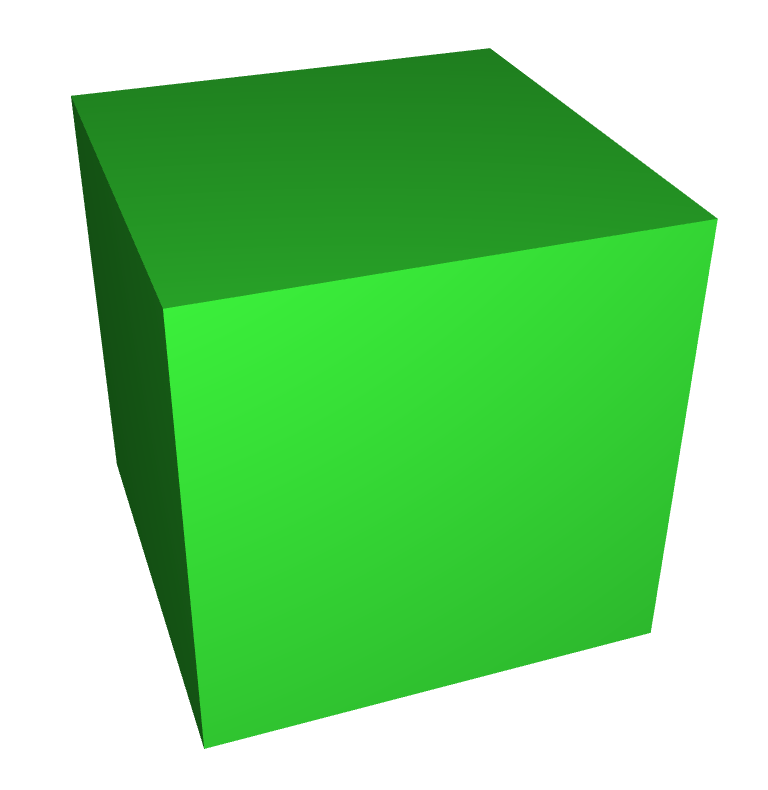
\includegraphics[width=0.3\textwidth]{images/cube.png}
                
\includegraphics[width=0.3\textwidth]{images/oct.png} \\
                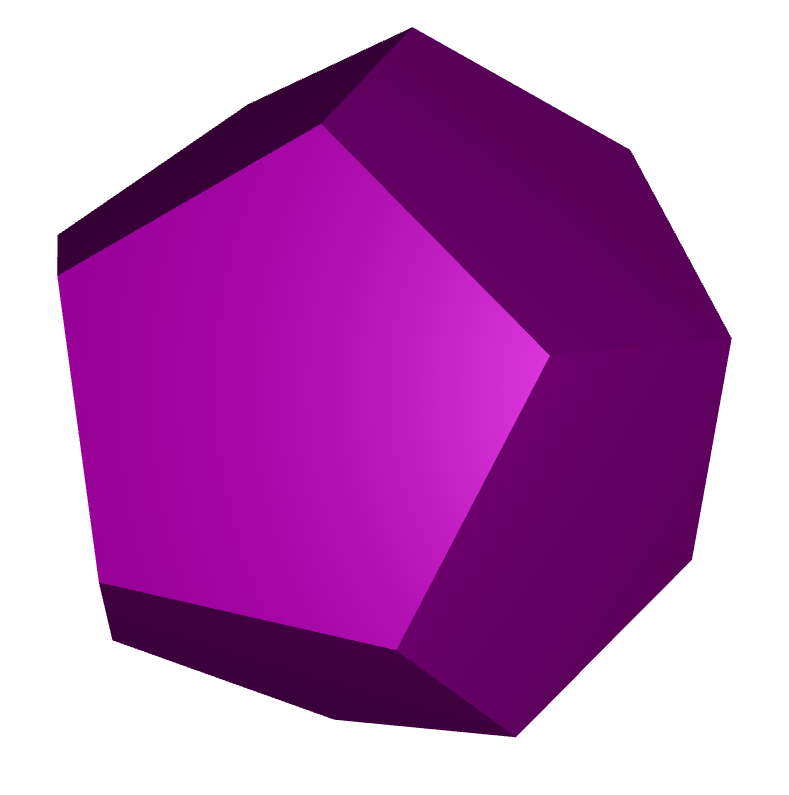
\includegraphics[width=0.3\textwidth]{images/dodec.png}
                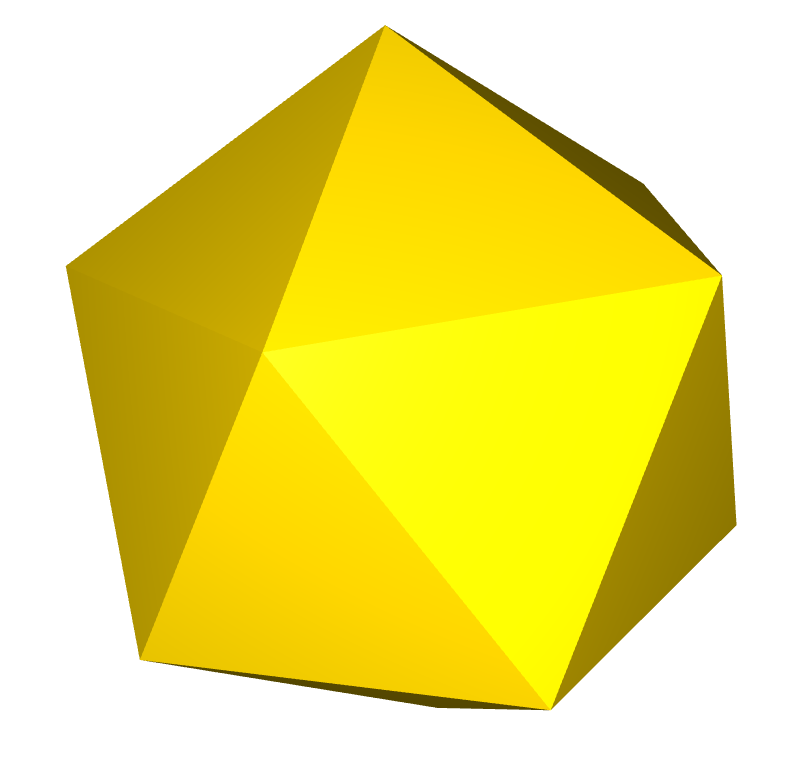
\includegraphics[width=0.3\textwidth]{images/ico.png}
            \end{column}
    \end{columns}
    \end{exampleblock}
\end{frame}

\begin{frame}
    \begin{block}{Bisherige Arbeiten}
        In \cite{GoertzenPhD} wurden solche Blöcke durch Deformation von \textbf{Fundamentalbereichen} von  \textbf{kristallographischer Gruppen} erzeugt.
    \end{block}
    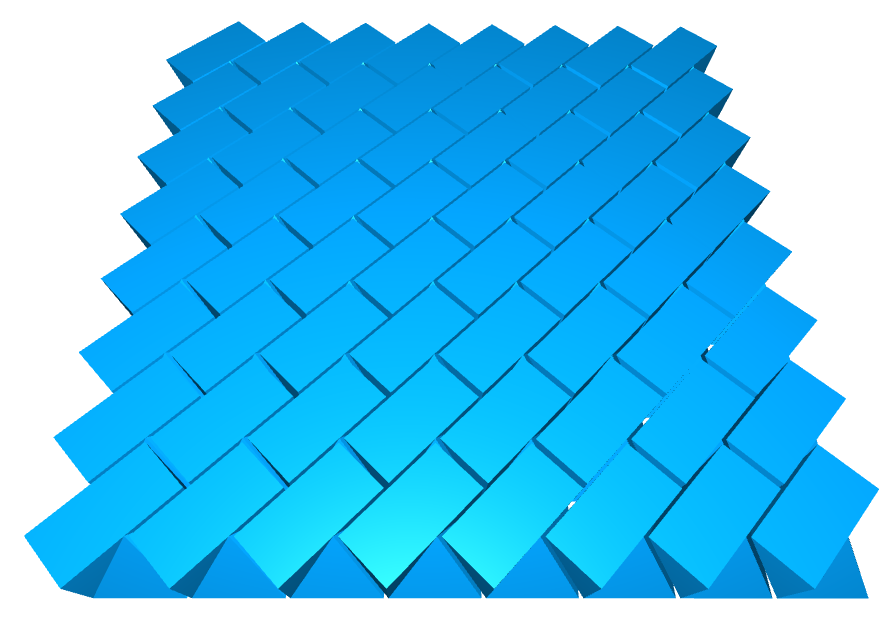
\includegraphics[width=0.48\textwidth]{images/p1.png}
    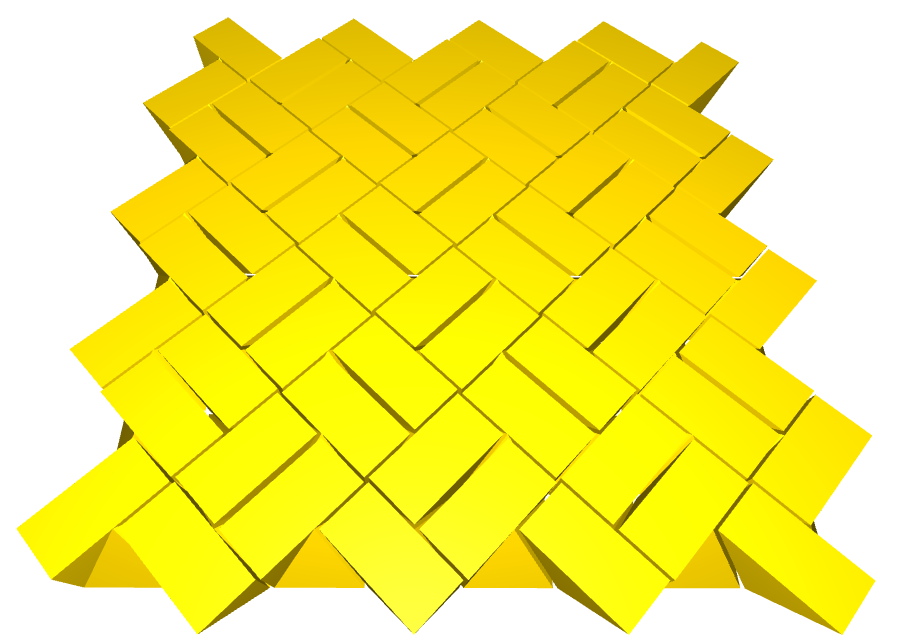
\includegraphics[width=0.48\textwidth]{images/p4.png}
\end{frame}

\section{Kristallographische Gruppen}
\begin{frame}
    \begin{notation}
        Seien $v, w \in \R^n$ Vektoren. \pause 
        Dann bezeichnen wir mit $d(v, w) \coloneqq ||v - w ||$ die Euklidische Distanz.
    \end{notation}
    \pause
    \begin{definition}
        Seien $n \in \N$ und $\phi: \R^n \to \R^n$. Dann bezeichnen wir $\phi$ als \emph{Isometrie}, falls für alle $v, w \in \R^n$:
        $$
            d(v^\phi, w^\phi) = d(v, w).
        $$\pause
        % Die Menge aller Isometrien zu einem festen $n$ bezeichnen wir mit $E(n)$.
        Weiterhin
        $$
            E(n) \coloneqq \{ \phi \mid \phi : \R^n \to \R^n \text{ Isometrie} \}.
        $$
    \end{definition}
\end{frame}

\begin{frame}
    \begin{remark}
        Sei $n \in \N$ fest. Dann
        \begin{itemize}[label=\textbullet]
            \item $(E(n), \circ)$ ist Gruppe, genannt \emph{Euklidische Gruppe},
            \item $E(n)$ wirkt auf $\R^n$.
        \end{itemize} 
    \end{remark}
    \pause
    \begin{notation}
        Sei $n \in \N$. Wir bezeichnen mit $O(n)$ die \emph{orthogonale Gruppe}. Diese ist isomorph zur Menge der orthogonalen $n \times n$ Matrizen.  
    \end{notation}
    
    
    % Dann ist die Menge aller Isometrien $E(n)$ eine Gruppe mit der Konkatenation von Abbildungen als Gruppenoperation.
    % Diese Gruppe bezeichnen wir als die \emph{euklidische Gruppe}. Die Gruppe operiert auf $\R^n$ durch die Anwendung eines Gruppenelements als Abbildung.
\end{frame}
% Bsp?
% system of representatives

\begin{frame}
    Es gilt, $E(n) \cong O(n) \ltimes \R^n$. D.h. für $\phi \in E(n)$ schreibe
    $$
        \phi = (\phi_o, \phi_t),
    $$
    wobei $\phi_o \in O(n)$ als \emph{orthogonaler Anteil} bezeichnet wird und $\phi_t \in \R^n$ als \emph{translatiorischer Anteil}. \\ \pause
    Betrachte $v \in \R^n$. Dann wirkt $\phi$ auf $v$ indem
    $$
        v^{(\phi_o, \phi_t)} = v^{\phi_o} + \phi_t.
    $$
\end{frame}

\begin{frame}
    \begin{block}{Beispiel}
        Betrachte
        $$
            p4 \coloneqq \langle \pi, \tau_1, \tau_2 \rangle
        $$
        wobei
        \begin{align*}
            \action<1->{
            &\pi = \left( \begin{pmatrix} 0 &1 \\ -1 &0\end{pmatrix}, \begin{pmatrix} 0 \\ 0 \end{pmatrix}\right),\\}
            \action<2->{&\tau_1 = \left( \begin{pmatrix} 1 &0 \\ 0 &1\end{pmatrix},\begin{pmatrix} 1 \\ 0 \end{pmatrix}\right), \\}
            \action<3->{&\tau_2 = \left( \begin{pmatrix} 1 &0 \\ 0 &1\end{pmatrix}, \begin{pmatrix} 0 \\ 1 \end{pmatrix}\right).}
        \end{align*}
    \end{block}
\end{frame}

\begin{frame}
    \only<1>{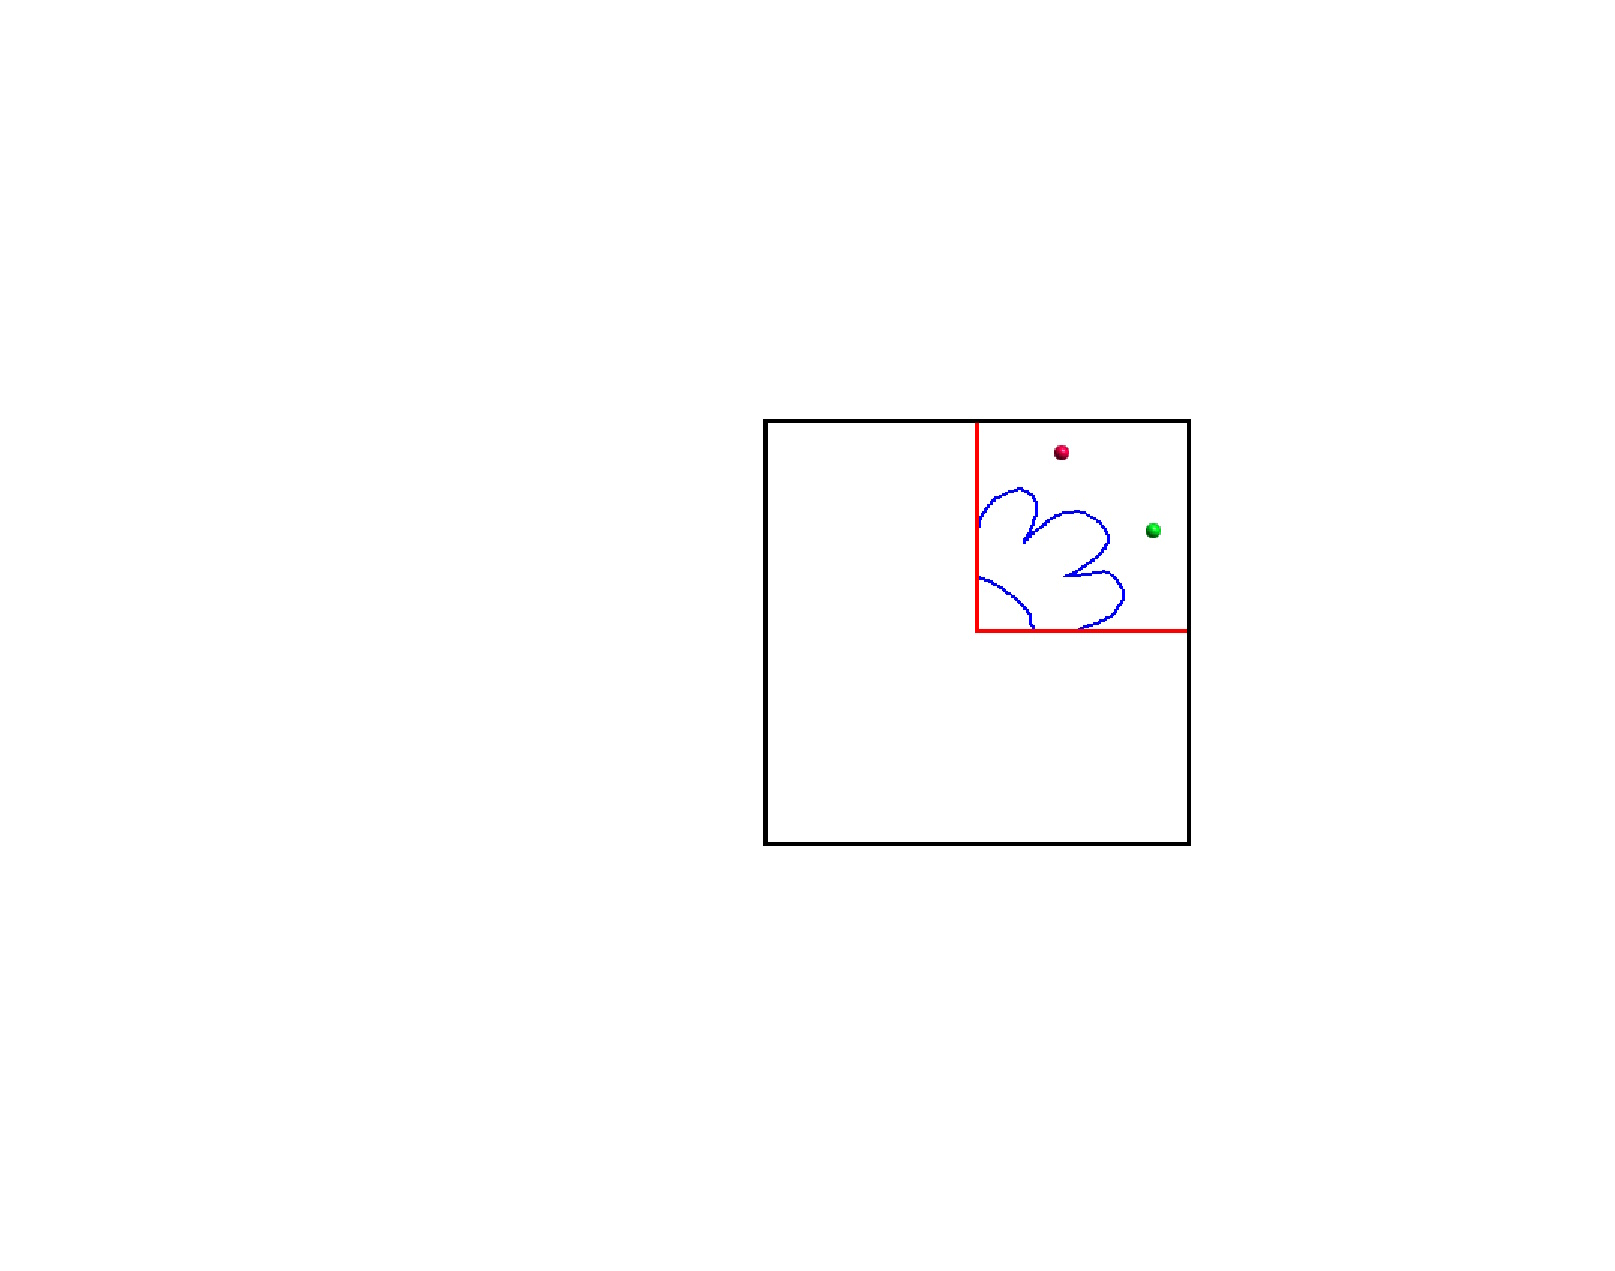
\includegraphics[width=\textwidth]{images/p4-animation/p4-no-rot.jpg}}
    \only<2>{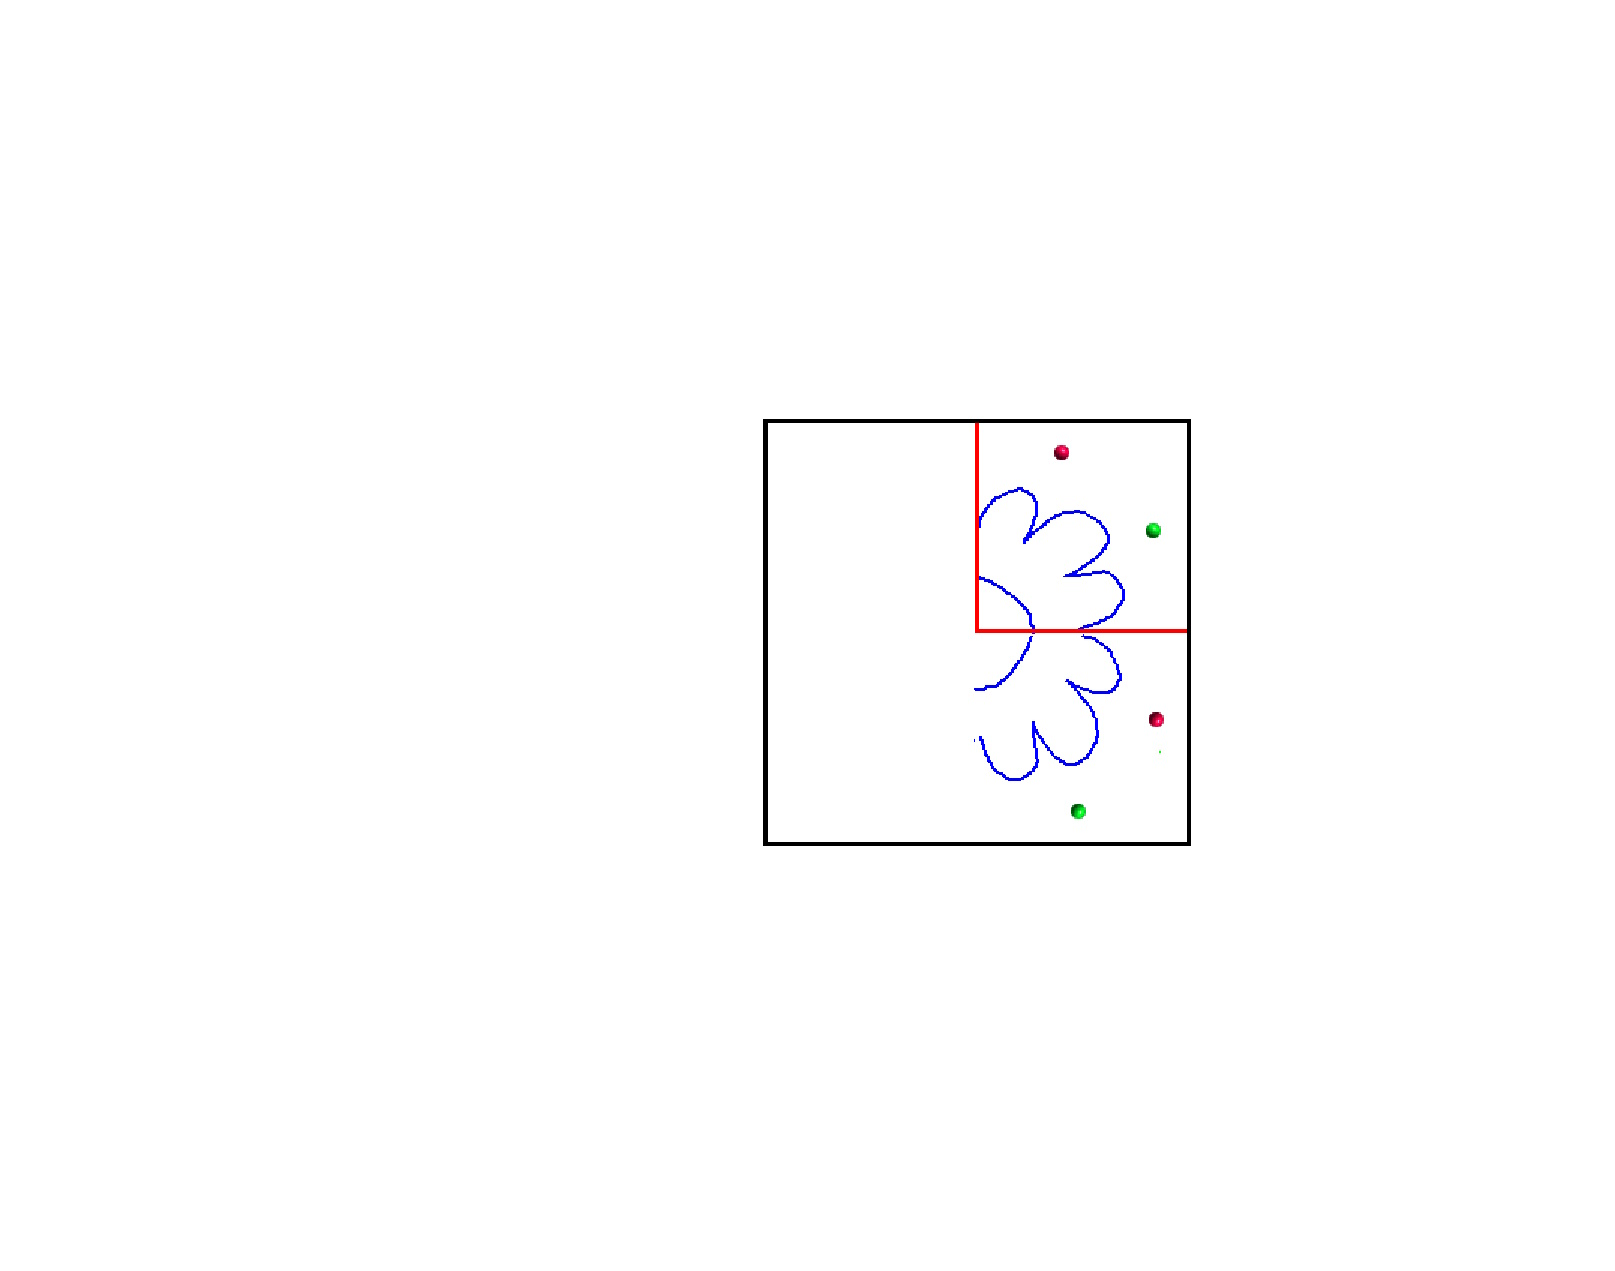
\includegraphics[width=\textwidth]{images/p4-animation/p4-one-rot.jpg}}
    \only<3>{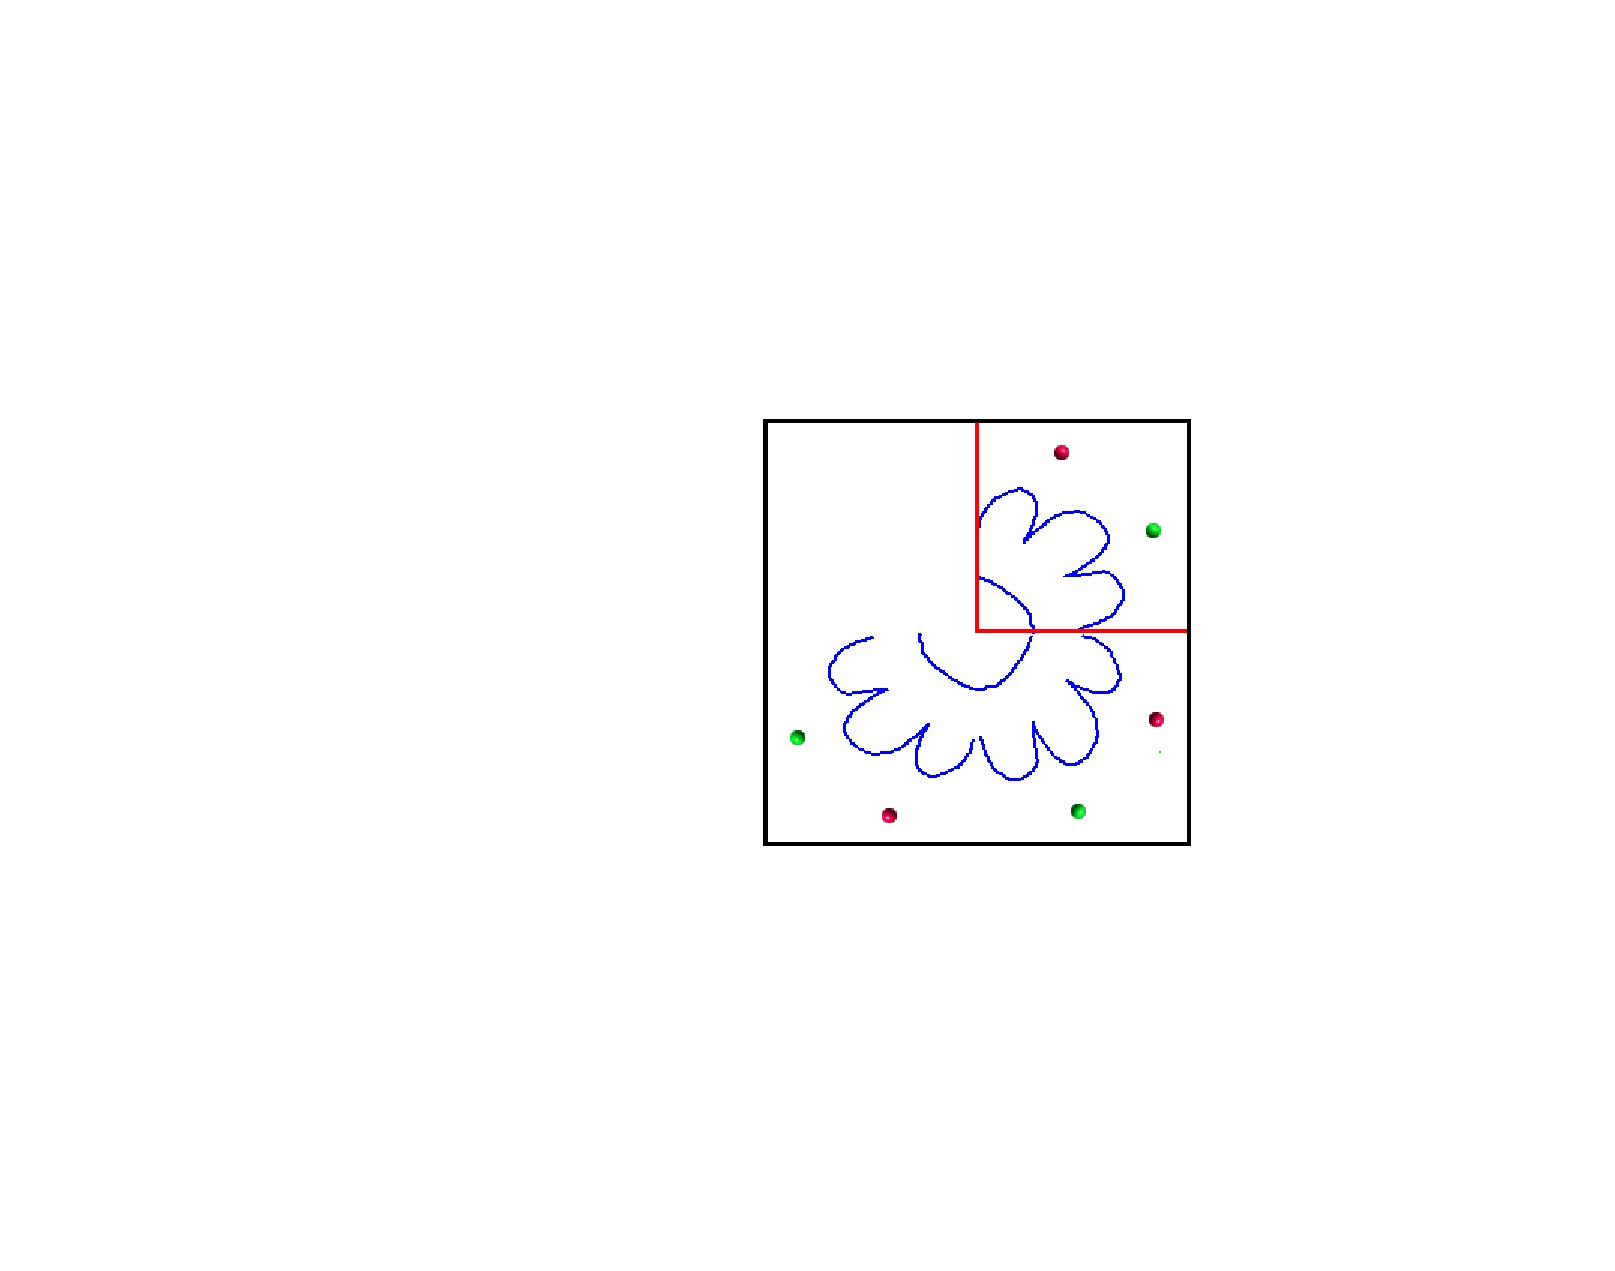
\includegraphics[width=\textwidth]{images/p4-animation/p4-two-rot.jpg}}
    \only<4>{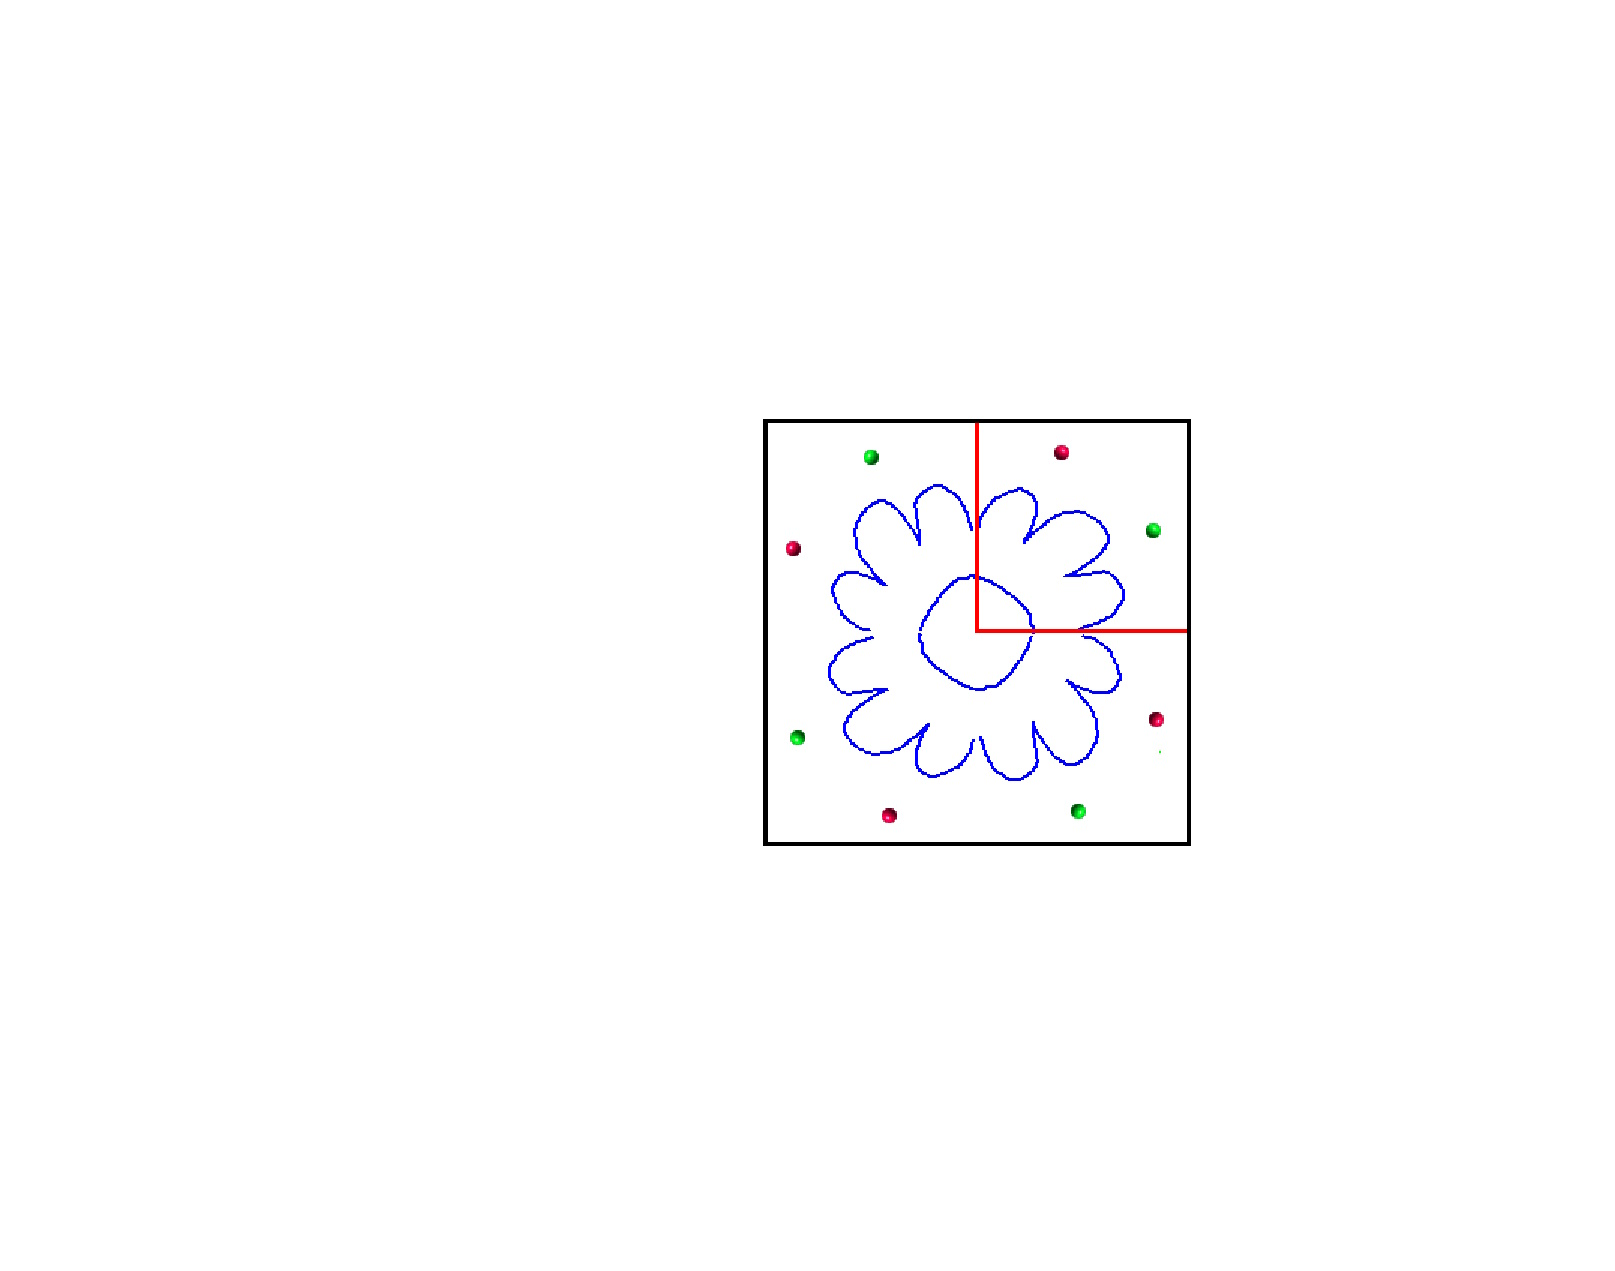
\includegraphics[width=\textwidth]{images/p4-animation/p4-full-rot.jpg}}
    \only<5>{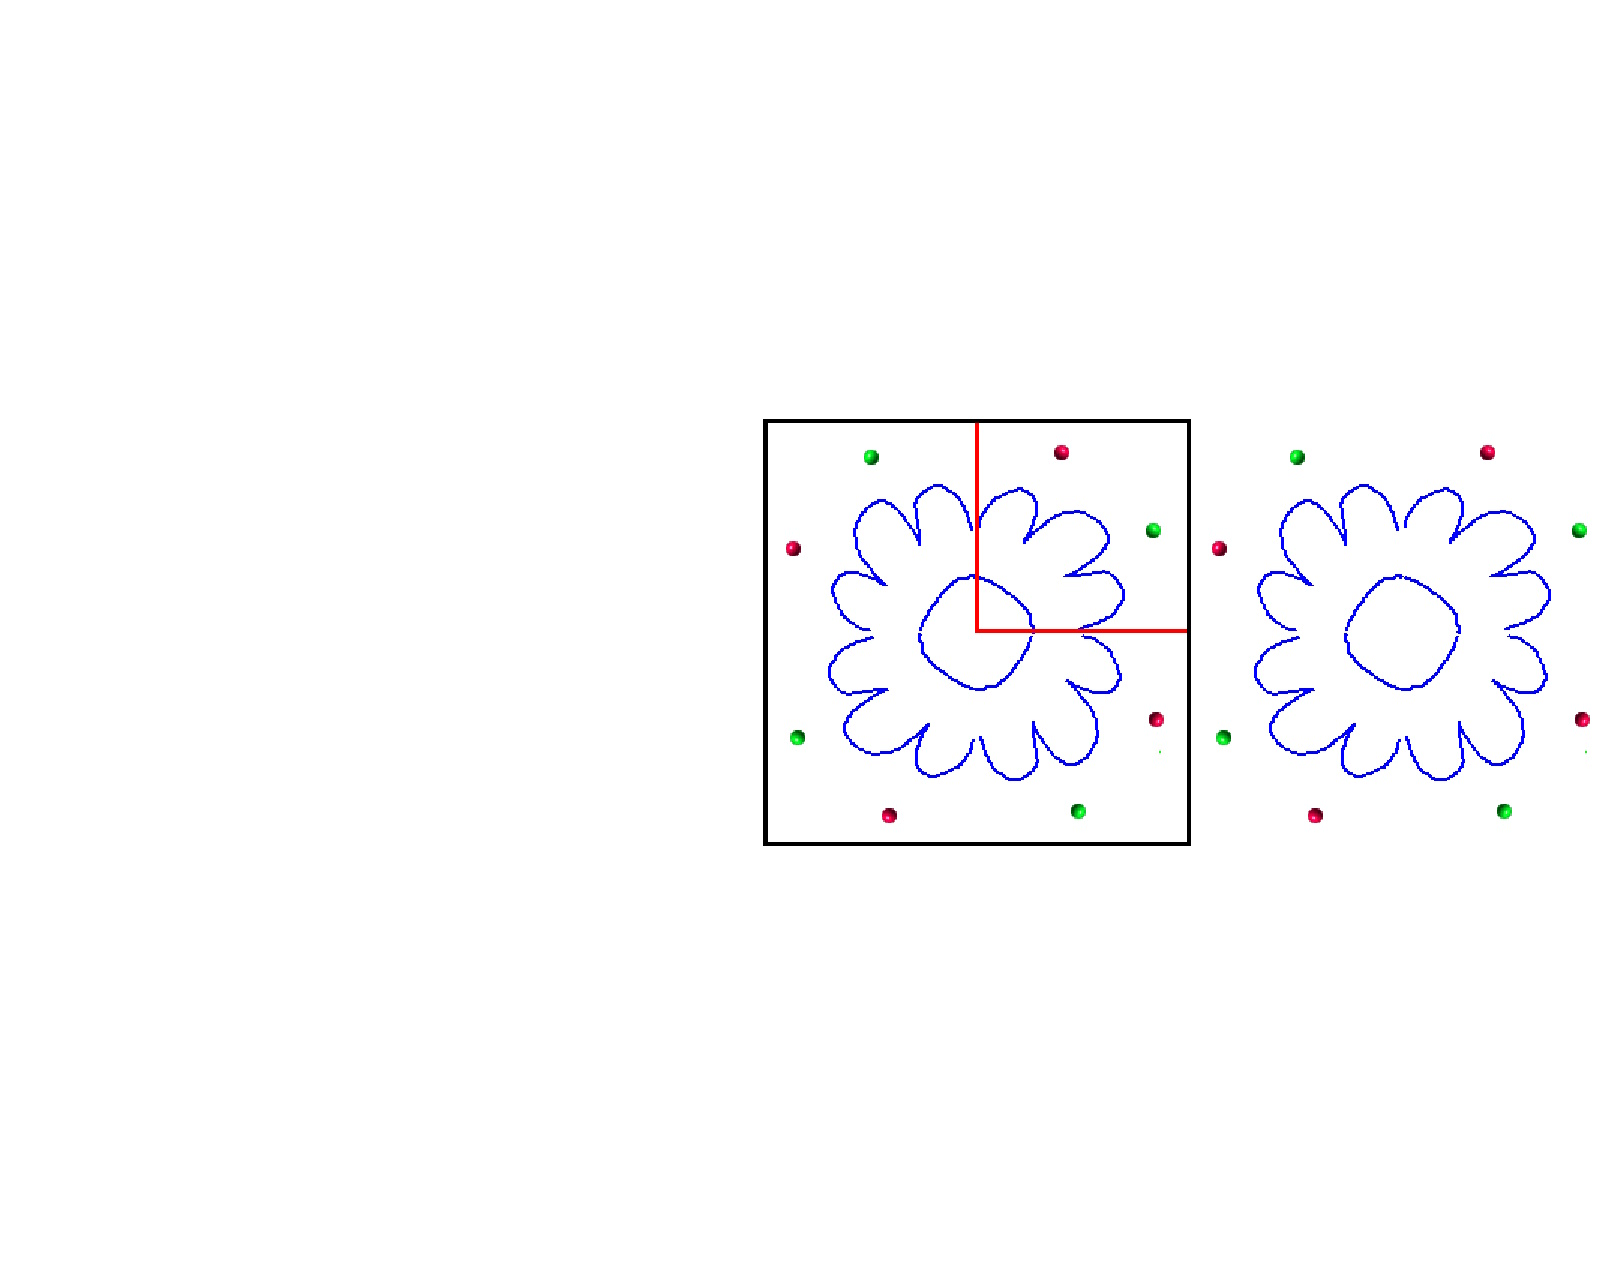
\includegraphics[width=\textwidth]{images/p4-animation/p4-one-trans.jpg}}
    \only<6>{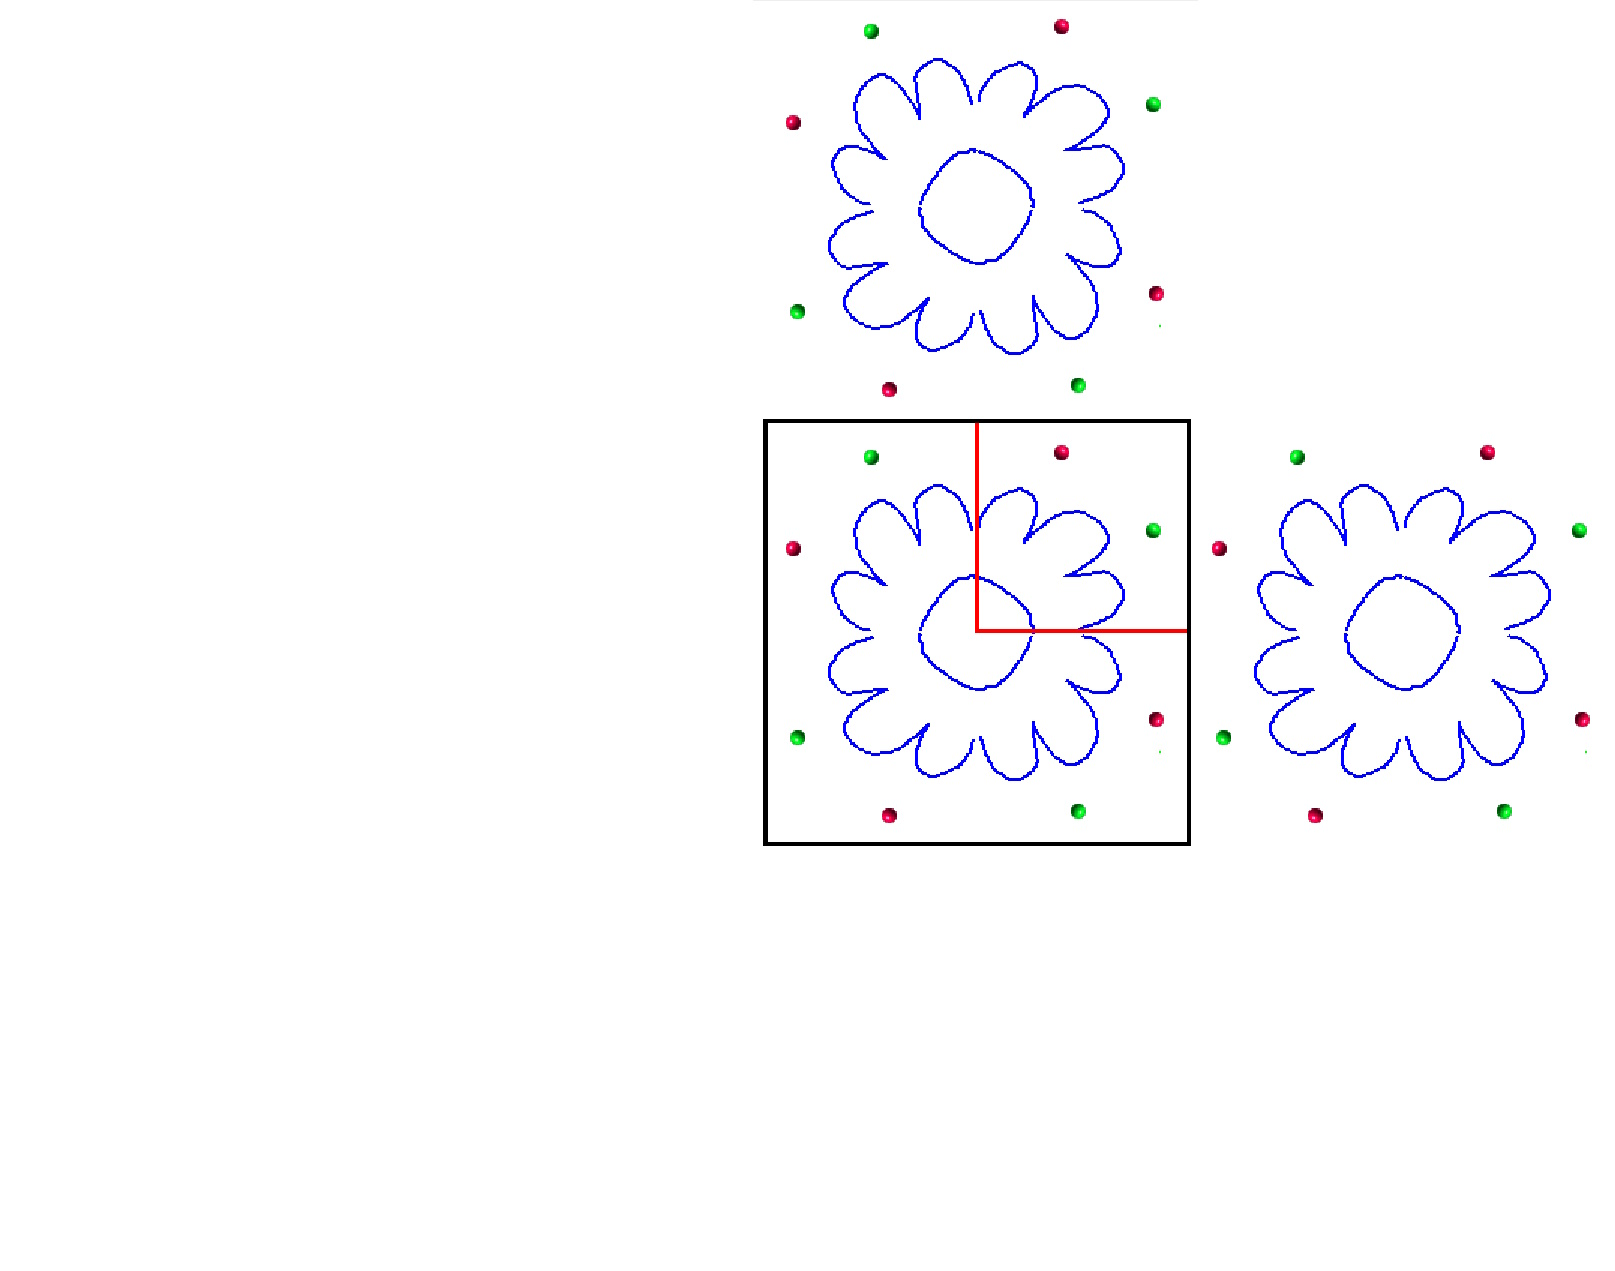
\includegraphics[width=\textwidth]{images/p4-animation/p4-two-trans.jpg}}
    \only<7>{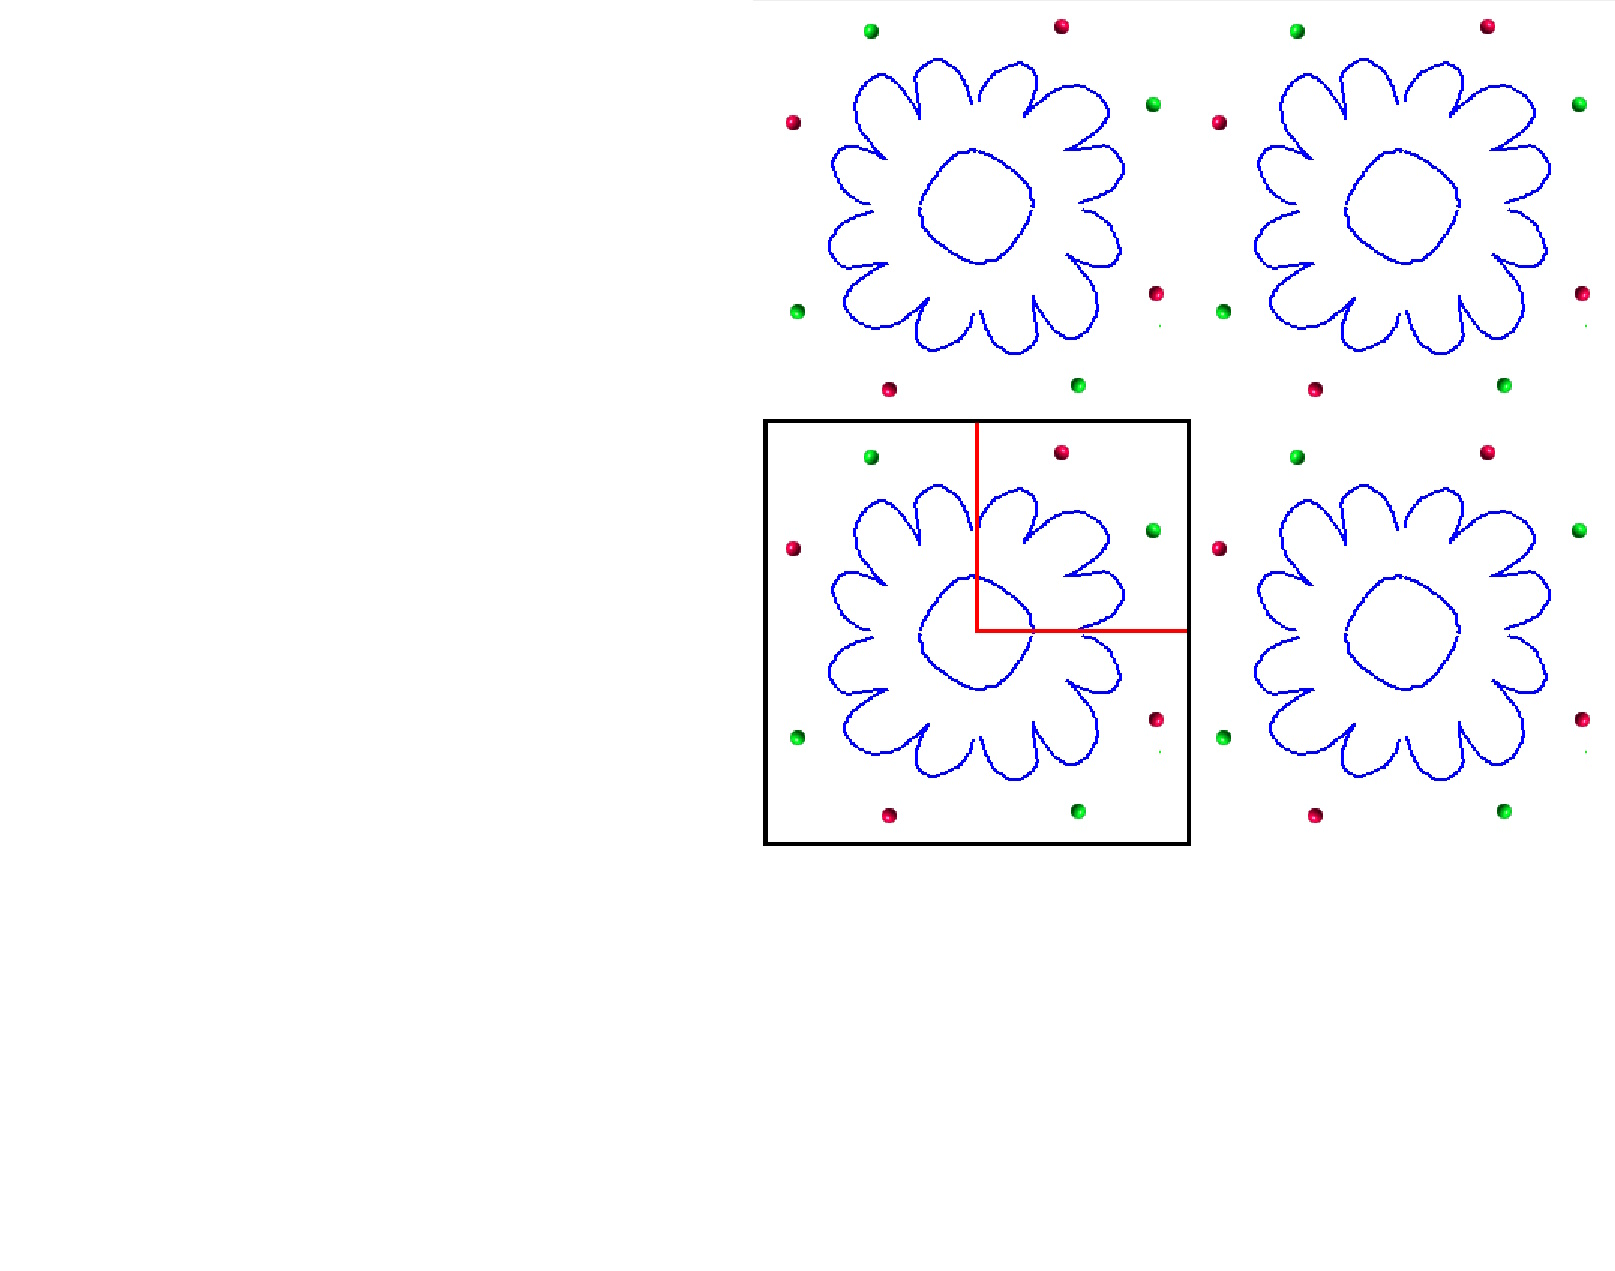
\includegraphics[width=\textwidth]{images/p4-animation/p4-three-trans.jpg}}
    \only<8>{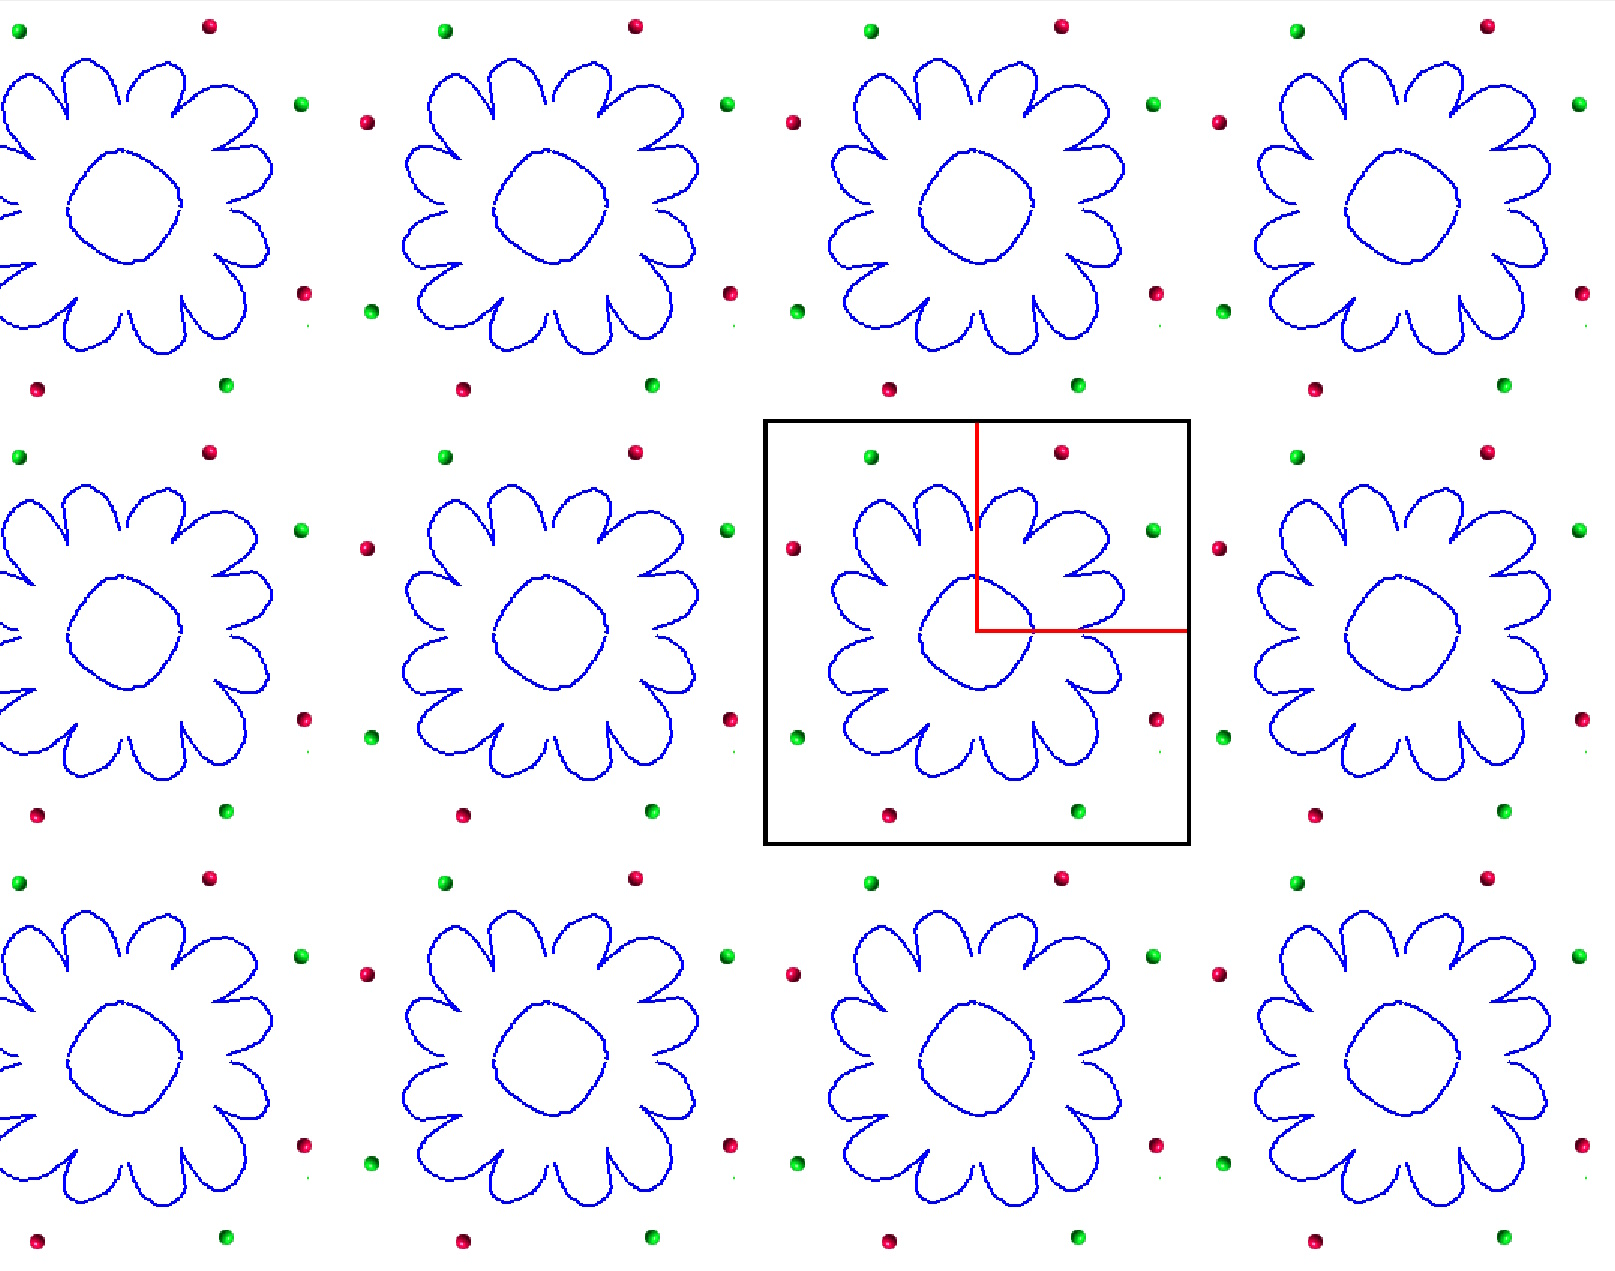
\includegraphics[width=\textwidth]{images/p4-animation/p4-full-trans.jpg}}
\end{frame}


\begin{frame}
    \only<1,3>{\begin{proposition}
        Sei $\Gamma \leq E(n)$ eine kristallographische Gruppe. Dann wird der \emph{Translationennormalteiler} von $\Gamma$ definiert als
        $$
            \T(\Gamma) \coloneqq \{ (\phi_o, \phi_t) \in \Gamma \mid \phi_o = Id \}.
        $$
        $\T(\Gamma)$ ist ein Normalteiler von $\Gamma$.
    \end{proposition}}
    \only<2>{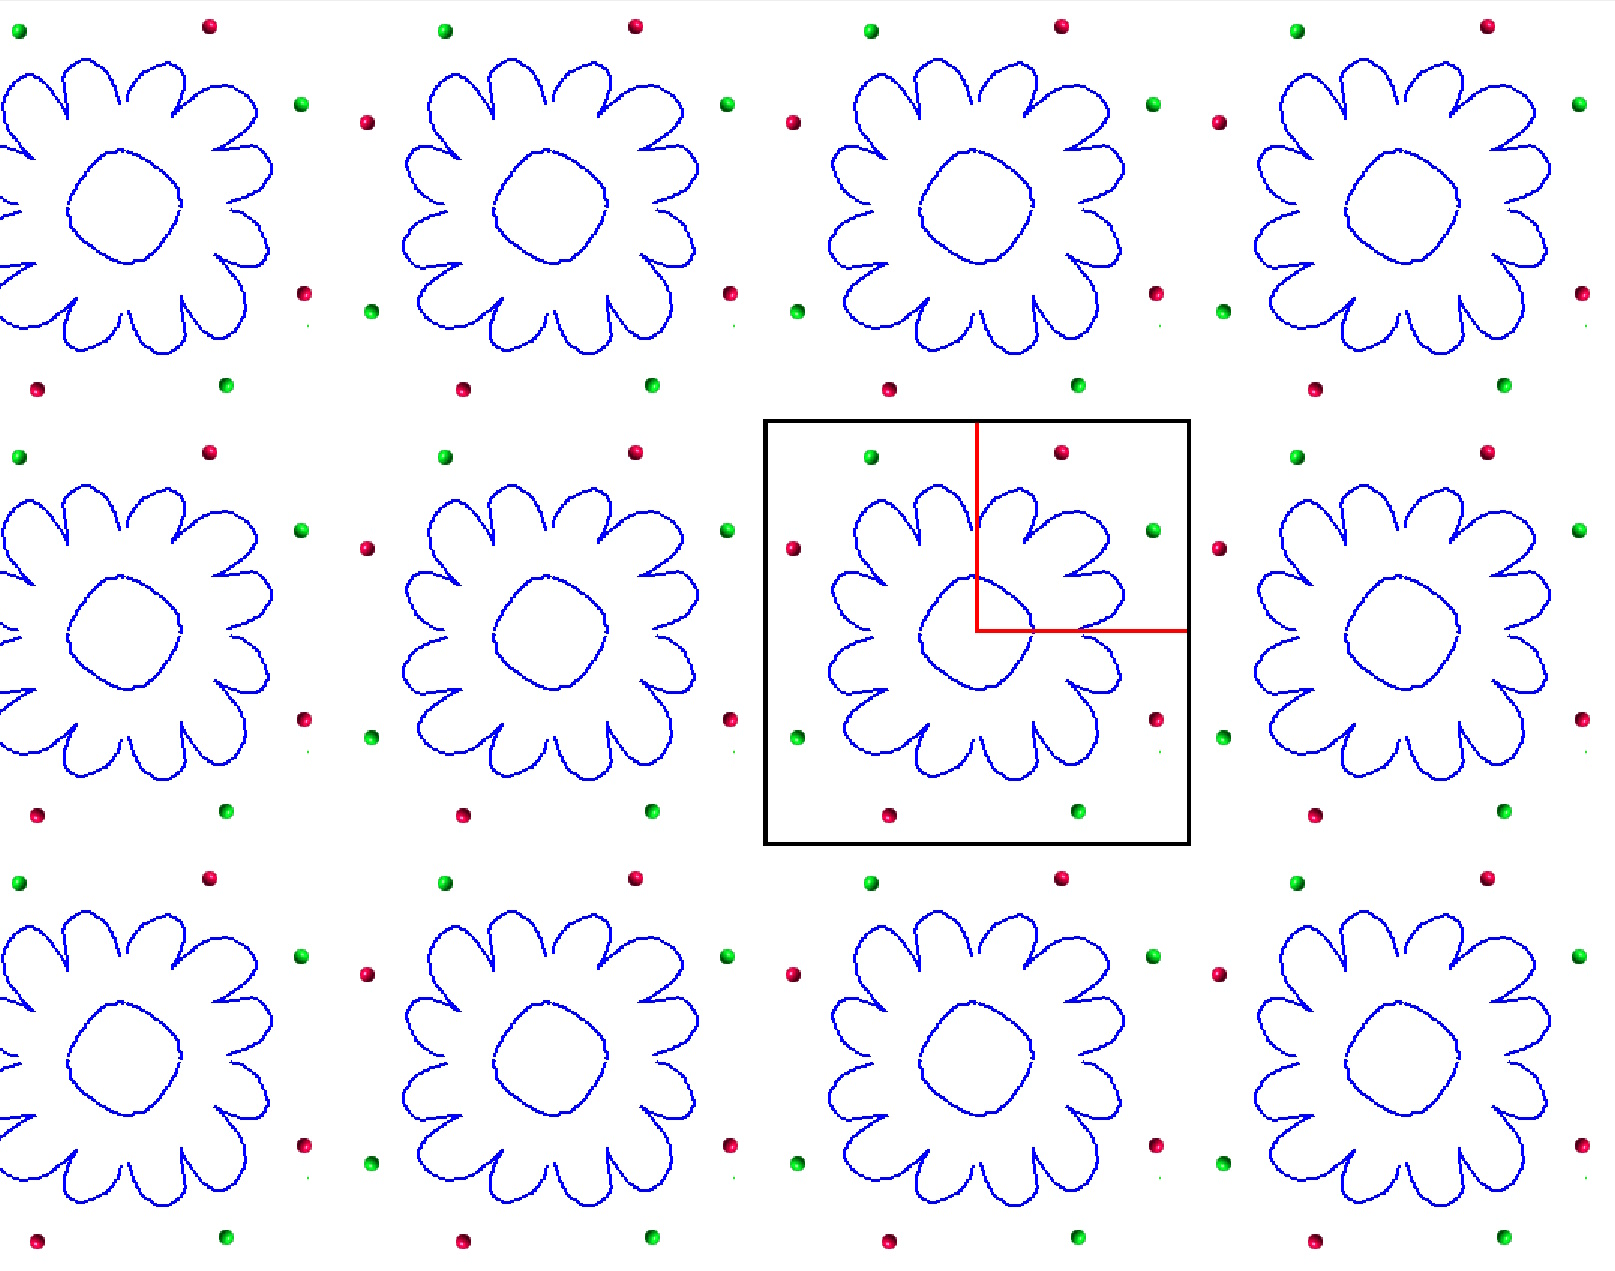
\includegraphics[width=\textwidth]{images/p4-animation/p4-full-trans.jpg}}
    \only<3>{\begin{definition}
        Sei $\Gamma \leq E(n)$ eine kristallographische Gruppe. Dann definieren wir die \emph{Punktgruppe} von $\Gamma$ als die Faktorgruppe
        $$
            \P(\Gamma) \coloneqq \Gamma / \T(\Gamma).
        $$
    \end{definition}}
\end{frame}

\begin{frame}
    \begin{proposition}
        Sei $\Gamma \leq E(n)$ eine kristallographische Gruppe. Die Menge 
        $$
            \L(\Gamma) \coloneqq \{ \phi_t \mid \phi \in \T(\Gamma) \}
        $$
        enthält $n$ linear unabhängige Vektoren. 
        % Diese bilden ein Gitter der Dimension $n$ und spannen sogenannte \emph{Translationszellen} auf.
    \end{proposition}
\end{frame}

\begin{frame}
    \centering
    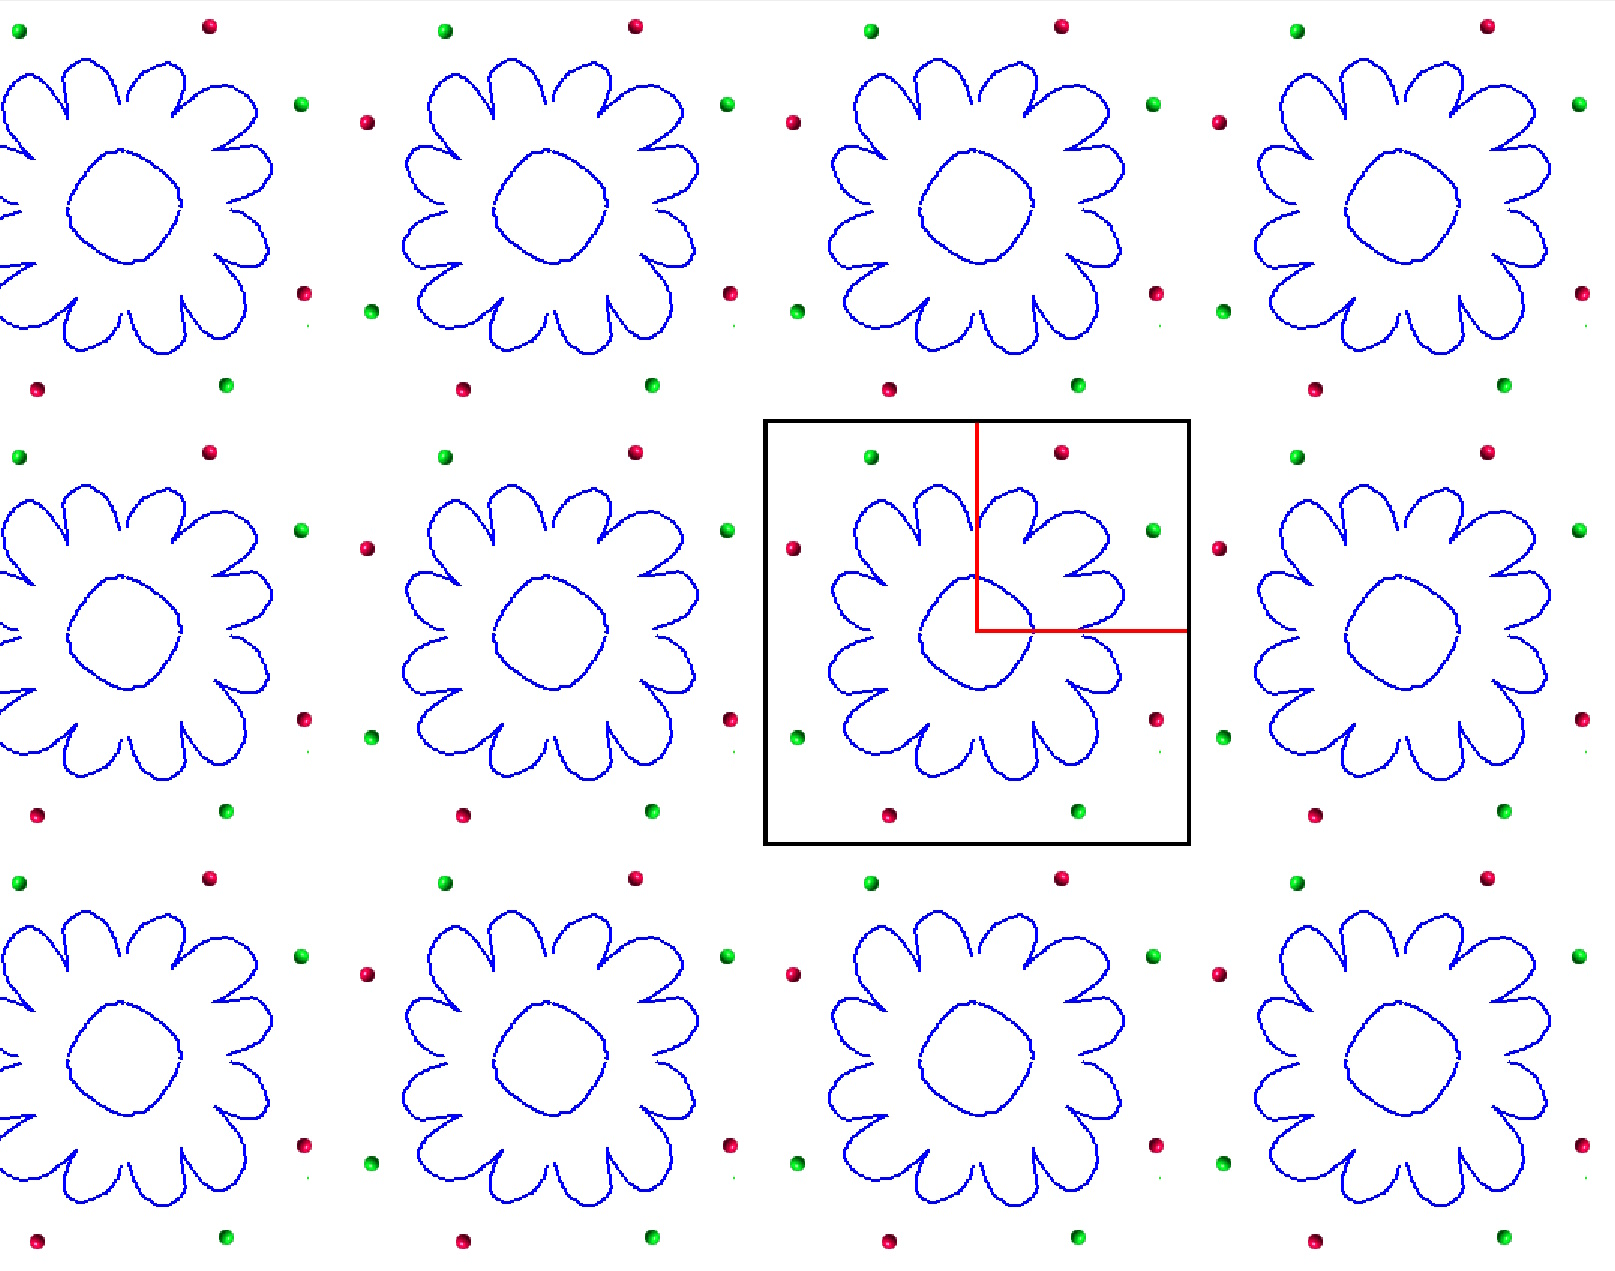
\includegraphics[width=\textwidth]{images/p4-animation/p4-full-trans.jpg}
\end{frame}

\begin{frame}
    \begin{definition}
        Sei $\Gamma \leq E(n)$ eine Untergruppe und $F \subseteq \R^n$ eine abgeschlossene Menge. Dann heißt $F$ ein \emph{Fundamentalbereich} von $\Gamma$ falls
        \begin{enumerate}[label=(\roman*)]
            \item $\bigcup_{\gamma \in \Gamma} F^\gamma = \R^n$\pause
            \item es gibt ein Vertretersystem $V \subseteq \R^n$ von den Bahnen der Operation von $\Gamma$ auf $\R^n$, sodass
                $$
                    F^\circ \subseteq V \subseteq F.
                $$
        \end{enumerate}
    \end{definition}

    \pause
    \begin{definition}
        Sei $\Gamma \leq E(n)$ eine Untergruppe. Dann heißt $\Gamma$ kristallographische Gruppe falls $\Gamma$ eine diskrete Untergruppe ist und ein kompakter Fundamentalbereich von $\Gamma$ existiert.
    \end{definition}
    In der Literatur werden kristallographische Gruppen (insbesondere der Dimension $3$) auch als Raumgruppen bezeichnet.
\end{frame}

\begin{frame}
    \centering
    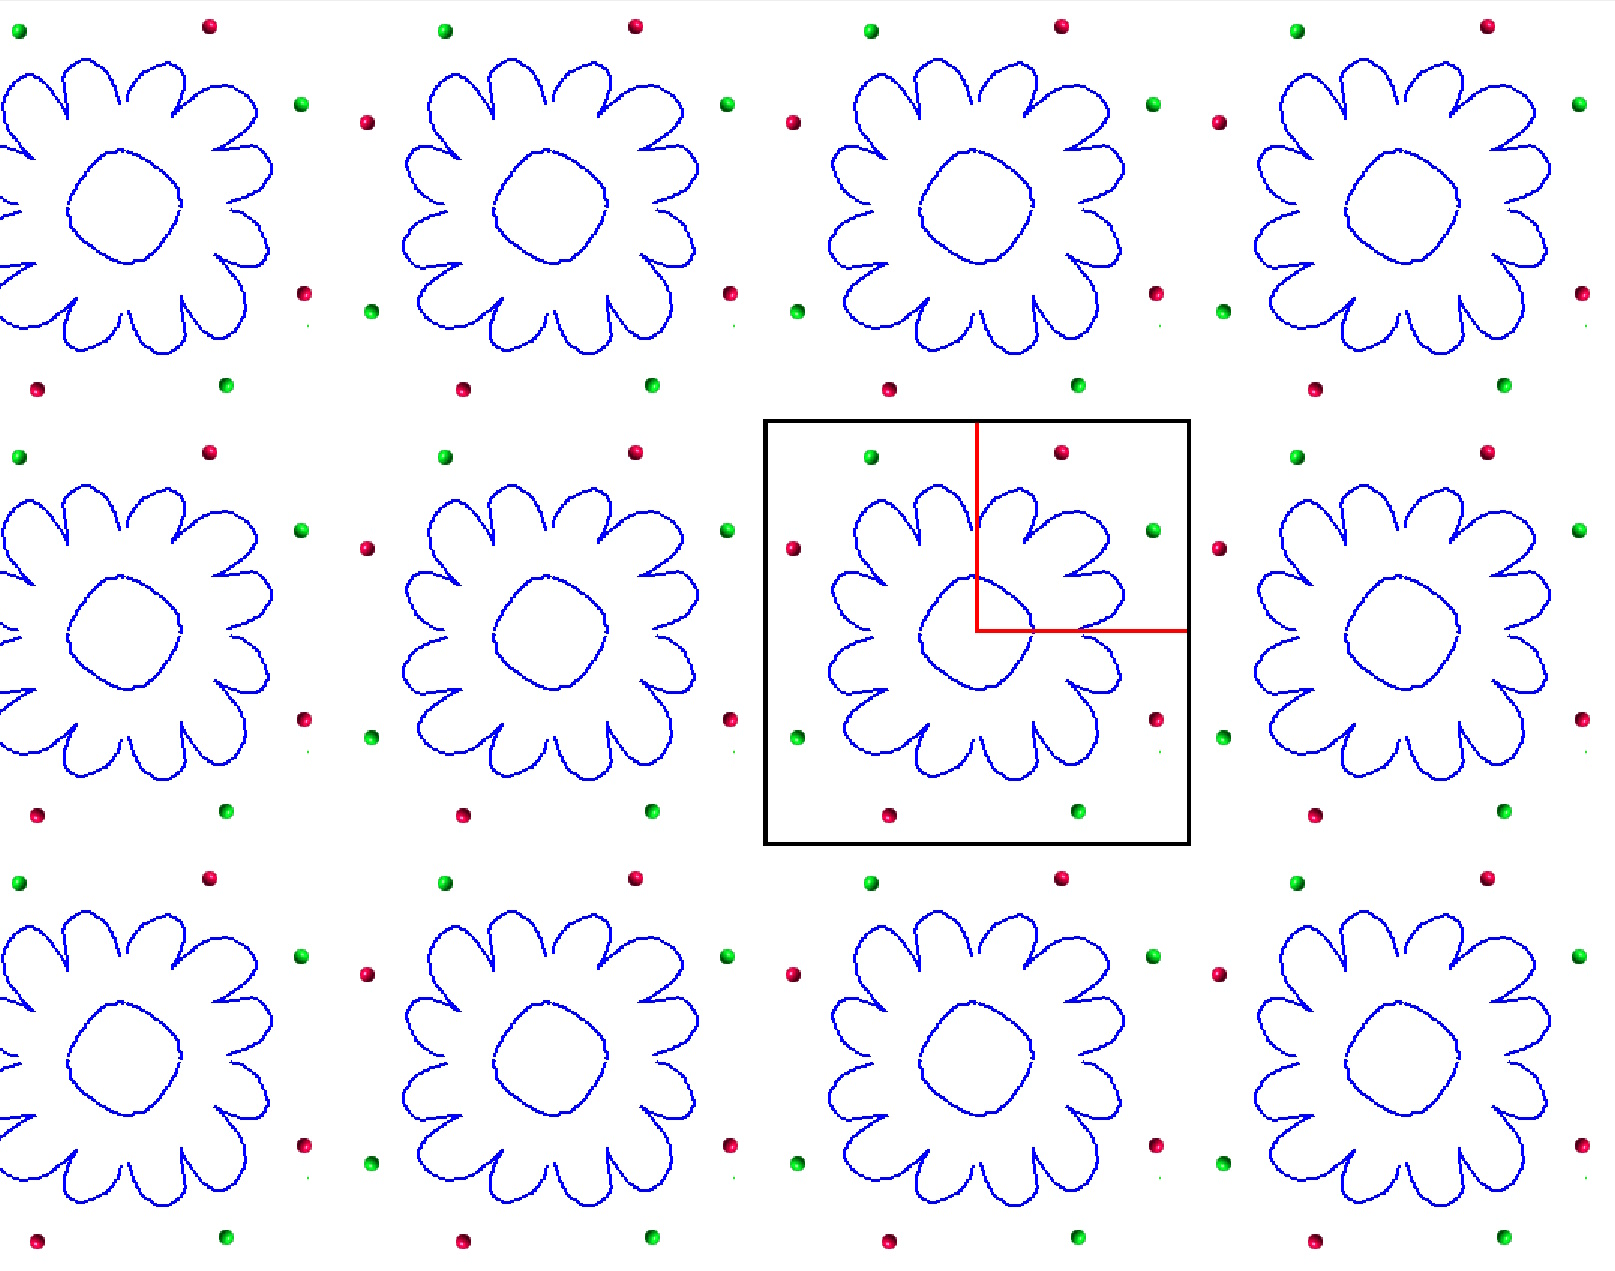
\includegraphics[width=\textwidth]{images/p4-animation/p4-full-trans.jpg}
\end{frame}

\begin{frame}
    In 1900 hat Hilbert 23 Probleme bei einem Kongress vorgestellt, die zu diesem Zeitpunkt ungelöst waren. \pause
    \begin{block}{18. Hilbert Problem}
        Gibt es für festes $n$ \textbf{endlich} viele kristallographische Gruppen?
    \end{block}
    \pause
    \begin{exampleblock}{Bieberbachsche Sätze (1910)}
        \textbf{Ja}, für festes $n \in \N$ gibt es nur endlich viele kristallographische Gruppen. \\
        Für $n=2$ gibt es $17$, für $n=3$ gibt es $230$.
    \end{exampleblock}
    Für bis niedrige Dimensionen sind alle dieser Gruppen bekannt, z.B. für $n\leq 4$ hier: \cite{crystGrpsDimFour}.
\end{frame}

% \begin{frame}
%     \centering
%     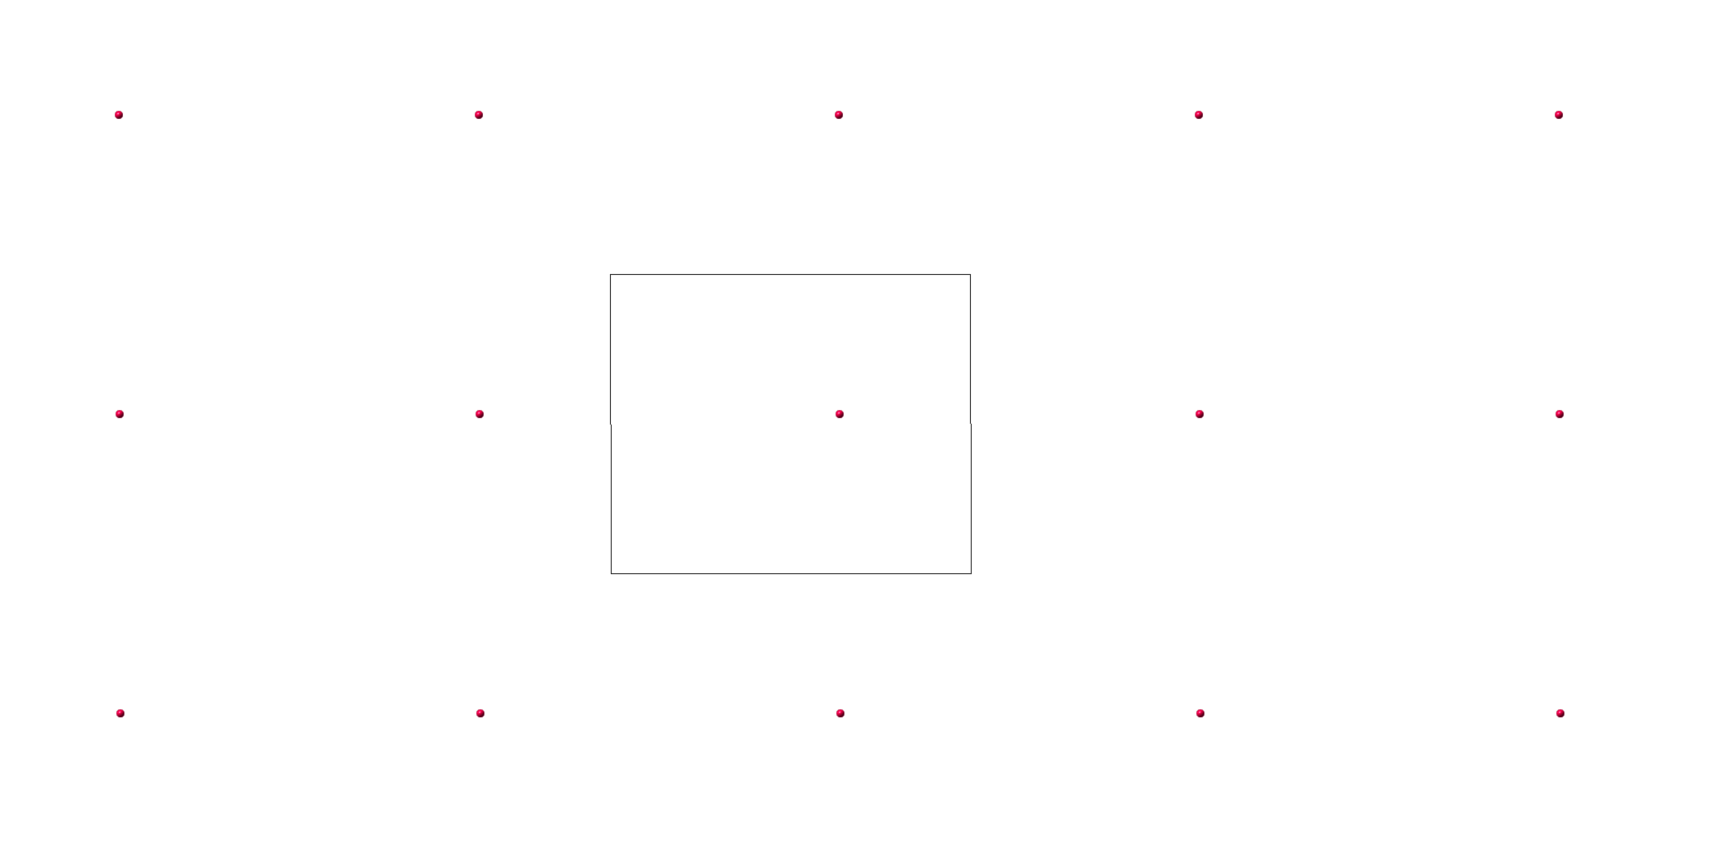
\includegraphics[width=\textwidth]{images/p1-escher.png}
% \end{frame}

% \begin{frame}
%     \centering
%     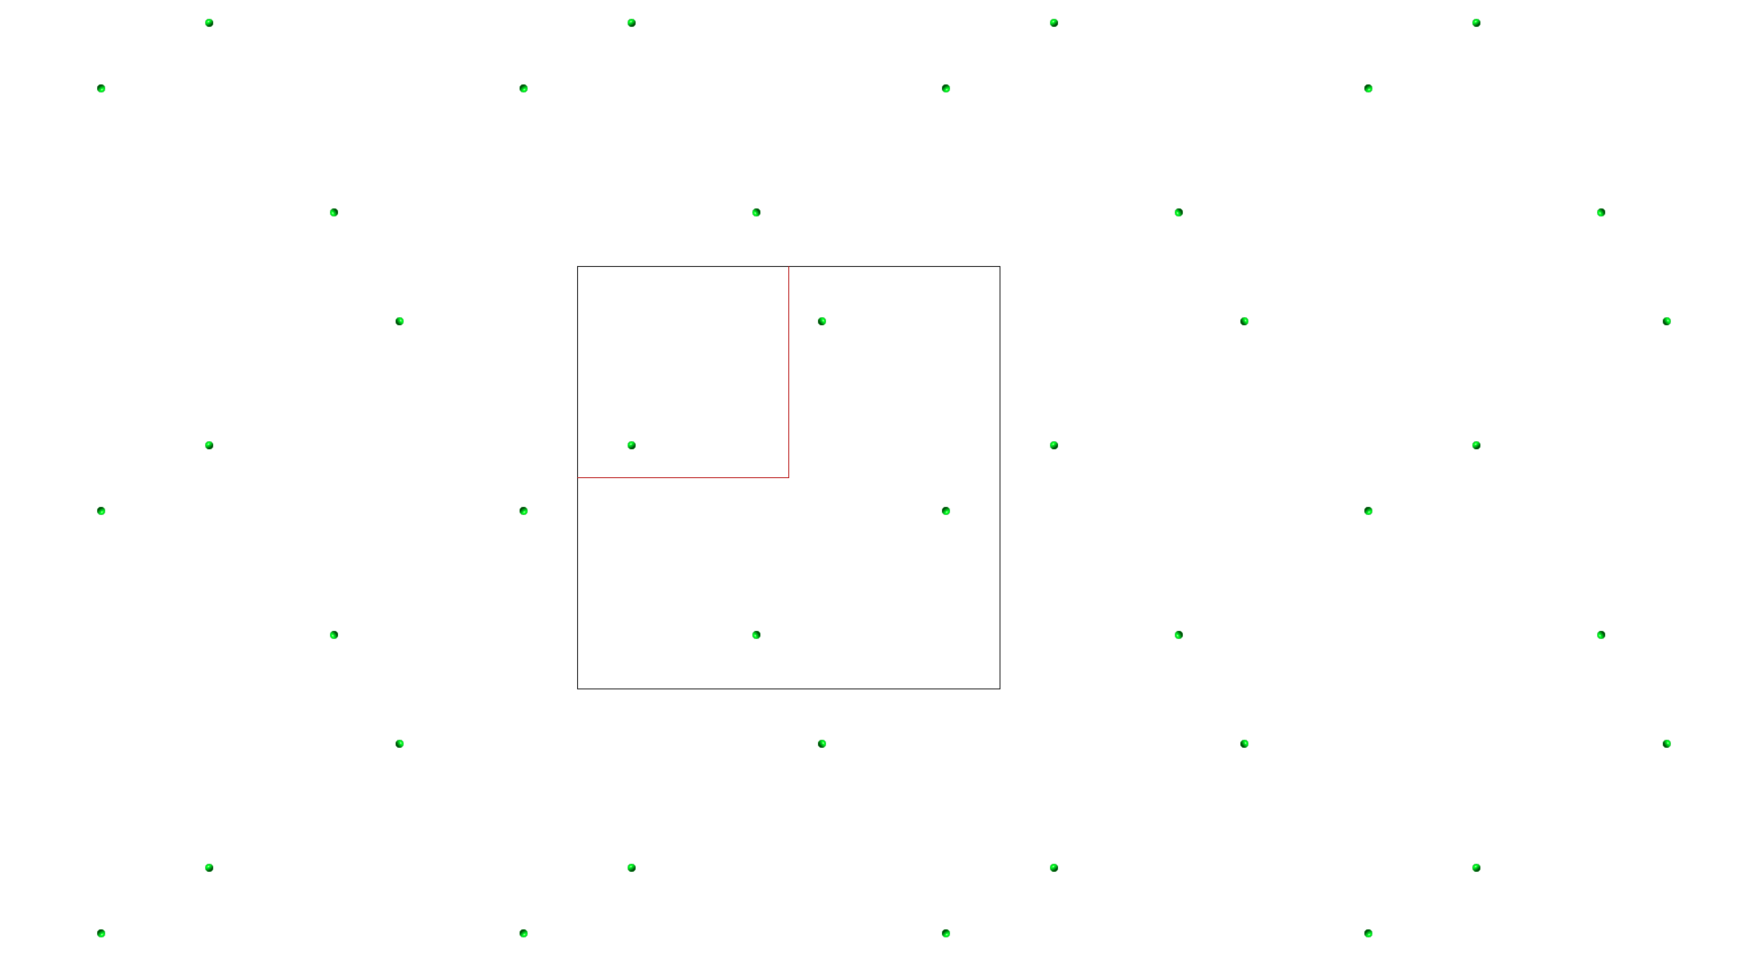
\includegraphics[width=\textwidth]{images/p4-escher.png}
% \end{frame}

% translationszelle?
\begin{frame}
    \begin{theorem}
        Sei $\Gamma$ eine kristallographische Gruppe mit Fundamentalbereich $F$ und Translationszelle $C$. Dann gilt
        $$
            vol(F) = \frac{vol(C)}{|\P(\Gamma)|}
        $$
    \end{theorem}
\end{frame}

\section{Dirichletzellen}
\begin{frame}
    \begin{alertblock}{Problem}
        Gegeben eine kristallographische Gruppe $\Gamma \leq E(n)$ durch ein endliches Erzeugendensystem. Wie kann ein Fundamentalbereich berechnet werden?
    \end{alertblock}
    \pause
    \begin{exampleblock}{Antwort}
        Hier: Algorithmus für Dirichletzellen
    \end{exampleblock}
\end{frame}

% \begin{frame}
%     \begin{definition}
%         Seien $u, v \in \R^n$ Vektoren. Wir nennen
%         $$
%             H^+(u, v) \coloneqq \{ w \in \R^n \mid d(u,w) \leq d(v, w) \}
%         $$
%         den \emph{Halbraum} von $u$ und $v$.
%     \end{definition}
%     \pause
%     \begin{definition}
%         Sei $O \subseteq \R^n$ eine diskrete Menge und $u \in O$ ein Punkt.
%         Dann nennen wir 
%         $$
% 		    D(u, O) \coloneqq \{ v \in \R^n \mid \forall w \in O \setminus \{ u \} : d(v, u) \leq d(v, w) \}
% 	    $$
%         die \emph{Dirichletzelle} von $u$ und $O$.
%     \end{definition} \pause
%     Oft nutzen wir die äquivalente Formulierung
%     $$
% 		D(u, O) = \bigcap_{w \in O, w \neq u} H^+(u, w).
% 	$$
% \end{frame}

% \begin{frame}
%     \centering
%     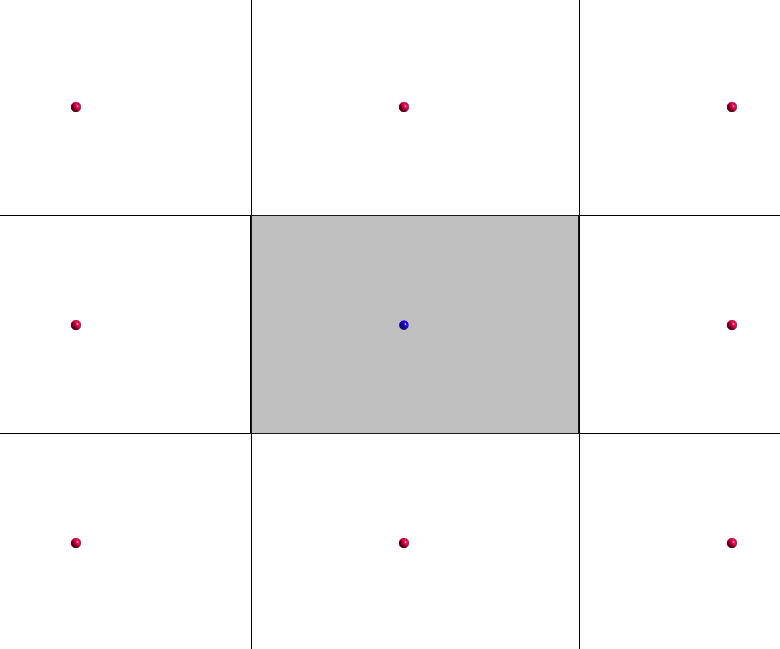
\includegraphics[width=0.7\textwidth]{images/dirichlet-example.png}
% \end{frame}

% \begin{frame}
%     \centering
%     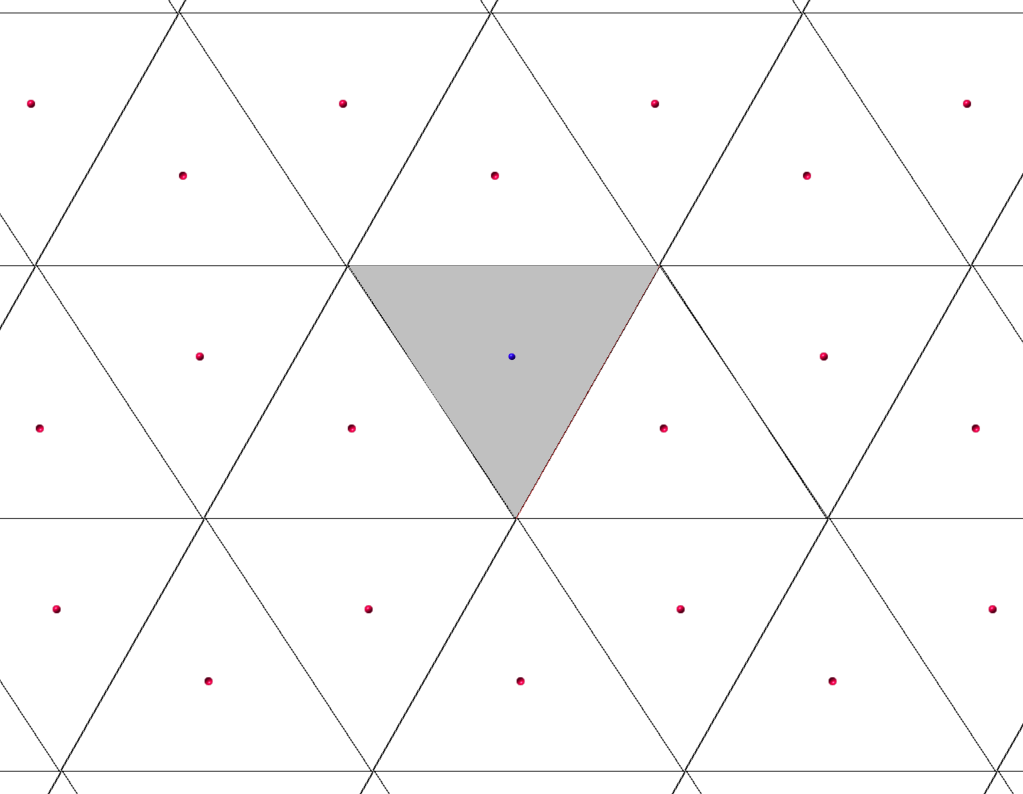
\includegraphics[width=0.7\textwidth]{images/p2-hex-dirichlet.png}
% \end{frame}

\begin{frame}
    % \begin{definition}
    %     Sei $\Gamma \leq E(n)$ eine kristallographische Gruppe und $v \in \R^n$ ein Vektor.
    %     Wir nennen $v$ in \emph{spezieller Lage} bzgl. $\Gamma$, falls 
    %     $$
    %         Stab_\Gamma(v) \neq \{Id\},
    %     $$
    %     sonst nennen wir ihn in \emph{allgemeiner Lage}.
    % \end{definition}
    % \pause
    \begin{theorem}[Dirichlet, {\cite[Thm. III.11 (ii)]{plesken1994}}]
        Sei $\Gamma \leq E(n)$ eine kristallographische Gruppe und $u \in \R^n$ in allgemeiner Lage. Dann ist 
        $$
            D(u, u^\Gamma) = \bigcap_{w \in u^\Gamma, w \neq u} H^+(u, w).
        $$ 
        ein Fundamentalbereich von $\Gamma$.
    \end{theorem}
\end{frame}

\begin{frame}
    \centering
    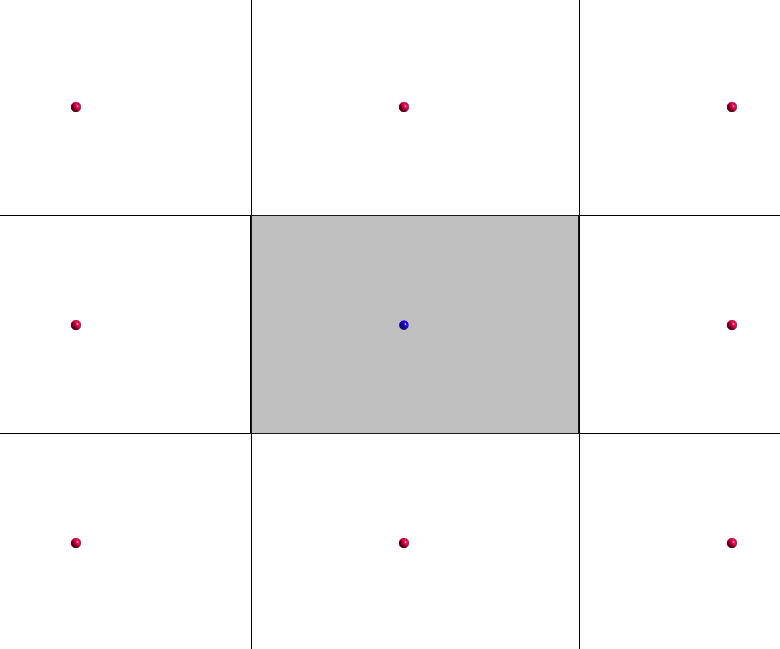
\includegraphics[width=0.8\textwidth]{images/dirichlet-example.png}
\end{frame}

\begin{frame}
    \centering
    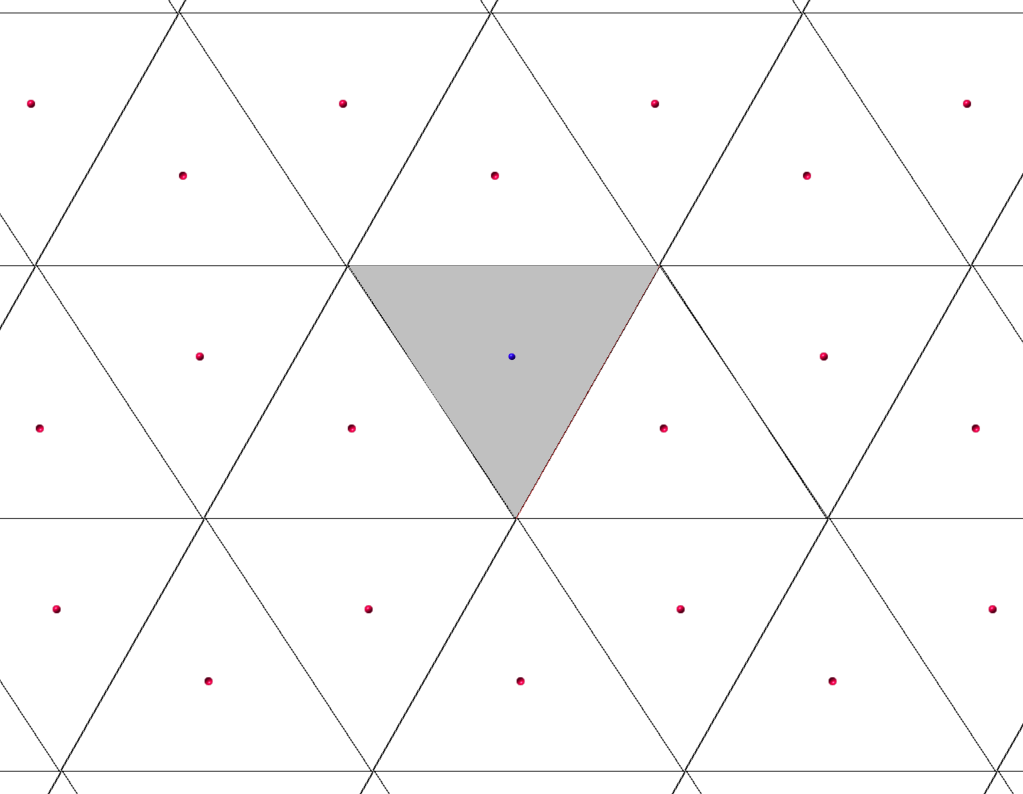
\includegraphics[width=\textwidth]{images/p2-hex-dirichlet.png}
\end{frame}

\section{Endliche Wortlänge}

\begin{frame}
    $$
        D(u, u^\Gamma) = \bigcap_{w \in u^\Gamma, w \neq u} H^+(u, w).
    $$ 
    \begin{alertblock}{Problem}
        $u^\Gamma$ ist unendlich.
    \end{alertblock}
\end{frame}

\begin{frame}
    \begin{block}{Idee}
        Halbräume die von zwei weit entfernten Punkten aufgespannt werden, haben weniger Einfluss als Halbräume, die von nahe beieinander liegenden Punkten aufgespannt werden.
    \end{block}
    \pause
    \begin{block}{Ansatz}
        Betrachte nur Isometrien, die einen Punkt nicht "zu weit weg" operieren.
    \end{block}
\end{frame}

% \begin{frame}
%     \begin{notation}
%         Sei $\Gamma \leq E(n)$ eine kristallographische Gruppe mit Fundamentalbereich $F$. Dann wählen wir Erzeugende von $\Gamma$ und $I, K$ endliche Indexmengen sodass
%         $$
%             \Gamma = \langle \rho_i, \tau_k \mid i \in I, k \in K \rangle,
%         $$
%         wobei $\tau_k \in \T(\Gamma)$ für alle $k \in K$ und für alle $i \in I$ sei $\rho_i \in \Gamma$ so gewählt, dass
%         $$
%             \Gamma = \bigcup_{i \in I} \rho_i \tau(\Gamma).
%         $$
%     \end{notation}

% \end{frame}

\begin{frame}
    \centering
    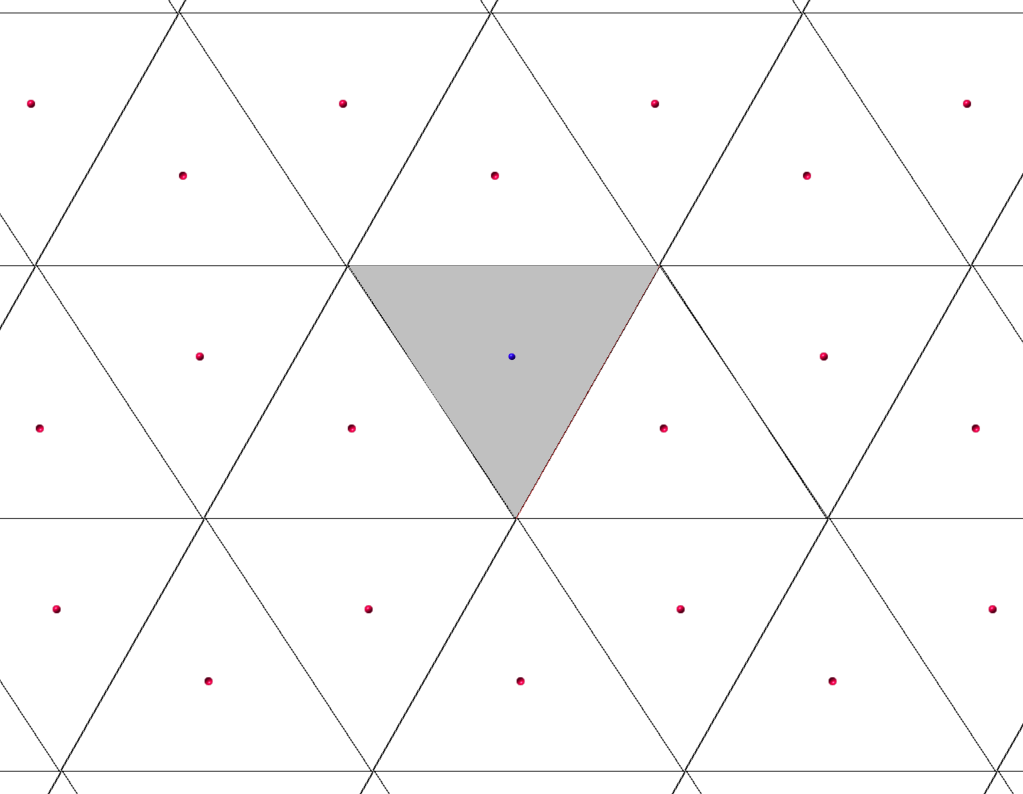
\includegraphics[width=\textwidth]{images/p2-hex-dirichlet.png}
\end{frame}

% angeben, dass neu?
\begin{frame}
    \begin{theorem}
        Sei $\Gamma \leq E(n)$ kristallographische Gruppe und $u \in \R^n$. Dann existiert ein $A \in \N$ sodass die Dirichletzelle $D(u, u^\Gamma)$ berechnet werden kann, als Schnitt der Halbräume $H^+(u, u^\gamma)$ für $\gamma \in \Gamma$ Wörter der Länge maximal $A+1$.  
    \end{theorem} \pause
    Damit haben wir einen Zugang, um Fundamentalbereiche in endlichen Schritten (algorithmisch) zu bestimmen. Leider ist $A$ im Allgemeinen nicht einfach bestimmbar.
\end{frame}

\begin{frame}
    \scalebox{.8}{\begin{minipage}{1.33\textwidth}
    \begin{algorithm}[H]
        \caption{Dirichlet Zelle}\label{alg:dirichletcell}
        \LinesNumberedHidden
        \SetAlgoLined
        \KwData{eine kristallographische Gruppe $\Gamma \leq E(n)$ und $u \in \R^n$, ein Punkt in allgemeiner Lage, sowie eine Menge $gens$ an Erzeugern von $\Gamma$.}
        \KwResult{$triangularComplex$, ein Fundamentalbereich. }
    
        % $fundamentalVolume \gets $ Volumen eines Fundamentalbereichs\;
        % $currentWords \gets gens$
    
        % $currentElementsInOrbit \gets [ u^\gamma \mid \gamma \in gens ]$ \;
    
        % $currentHalfspaces \gets$ Halbräume $H_{u,v}$ für alle $v \in currentElementsInOrbit$\;
        $fundamentalDomainCandidate \gets$ gegeben durch Schnitt über $gens$\;
    
        \While{$vol(fundamentalDomainCandidate) < fundamentalVolume$}{
            % $currentWords \gets [currentWords, [word \cdot gen \mid word \in currentWords,  gen \in gens]]$\;
    
            % \For{ $\gamma \in currentWords$}{
            %     Add(currentElementsInOrbit, $u^\gamma$)\;
            % }
    
            % $currentHalfspaces \gets$ Halbräume $H_{u,v}$ für alle $v \in currentWords$\;
            $fundamentalDomainCandidate \gets$ gegeben durch Schnitt über Wortlänge $+1$\;
        }
    
        return $fundamentalDomainCandidate$\;
    \end{algorithm}
    \end{minipage}}
\end{frame}

% \begin{frame}
%     \scalebox{.8}{\begin{minipage}{1.33\textwidth}
%     \begin{algorithm}[H]
%         \caption{Dirichlet Cell}\label{alg:dirichletcell}
%         \LinesNumberedHidden
%         \SetAlgoLined
%         \KwData{eine kristallographische Gruppe $\Gamma \leq E(n)$ und $u \in \R^n$, ein Punkt in allgemeiner Lage, sowie eine Menge $gens$ an Erzeugern von $\Gamma$.}
%         \KwResult{$triangularComplex$, ein Fundamentalbereich. }
    
%         $fundamentalVolume \gets $ Volumen eines Fundamentalbereichs\;
%         $currentWords \gets gens$
    
%         $currentElementsInOrbit \gets [ u^\gamma \mid \gamma \in gens ]$ \;
    
%         $currentHalfspaces \gets$ Halbräume $H_{u,v}$ für alle $v \in currentElementsInOrbit$\;
%         $fundamentalDomainCandidate \gets$ gegeben durch Schnitt von $currentHalfspaces$\;
    
%         \While{$vol(fundamentalDomainCandidate) < fundamentalVolume$}{
%             $currentWords \gets [currentWords, [word \cdot gen \mid word \in currentWords,  gen \in gens]]$\;
    
%             \For{ $\gamma \in currentWords$}{
%                 Add(currentElementsInOrbit, $u^\gamma$)\;
%             }
    
%             $currentHalfspaces \gets$ Halbräume $H_{u,v}$ für alle $v \in currentWords$\;
%             $fundamentalDomainCandidate \gets$ gegeben durch Schnitt von $currentHalfspaces$\;
%         }
    
%         return $fundamentalDomainCandidate$\;
%     \end{algorithm}
%     \end{minipage}}
% \end{frame}

% \begin{frame}
%     \begin{block}{Erweiterungen}
%         \begin{itemize}[label=\textbullet]
%             \item Verifikation von 
%         \end{itemize}
%     \end{block}    
% \end{frame}

\section{Motivation}
\begin{frame}
    Bisher: zwei-dimensional.
    \begin{block}{Erweiterung}
         Alle Aussagen gelten für $n \in \N$. Damit erhalten wir Zugang zu den 230 drei-dimensionalen kristallographischen Gruppen.
    \end{block}
\end{frame}

\begin{frame}
    \begin{block}{Vorgehen}
        \begin{enumerate}[label=(\roman*)]
            \item Generiere Fundamentalbereich einer kristallographischen Gruppe
            \item Deformiere diesen Fundamentalbereich
            \item Prüfe ob topologisches Interlocking vorliegt
        \end{enumerate}
    \end{block}
\end{frame}

\begin{frame}
    \begin{exampleblock}{Anwendungen}
        \begin{itemize}[label=\textbullet]
            \item doppelt gekrümmte Baugruppen
            \item i.A. nicht planare Baugruppen
            \item füllung spezieller Formen
            \item materialminimerte Kraftabtragung
        \end{itemize}
    \end{exampleblock}
\end{frame}

\begin{frame}
    \begin{block}{Offene Themen}
        \begin{itemize}[label=\textbullet]
            \item Verbesserung/Nachweis der (optimimalität) der Schranken
            \item Allgemeine Verfügbarkeit in einer Software
            \item Charakterisierung wann topologische Interlockings entstehen
            \item Charakterisierung welche topologische Interlockings "gut" sind
        \end{itemize}
    \end{block}
\end{frame}


\begin{frame}
    \begin{center}
        Vielen Dank für die Aufmerksamkeit \\ 
        Gibt es Fragen?
    \end{center}
    \vspace{1em}
    \hrule
    \vspace{1em}
    Referenzen:
    \printbibliography
\end{frame}

\end{document}
